% Chapter Electrodes

\chapter{Electrodes Design with Electrostatic Simulation} % Main chapter title

\label{ChapterElectrodes} % Change X to a consecutive number; for referencing this chapter elsewhere, use \ref{ChapterX}

%----------------------------------------------------------------------------------------
%	BEGING CHAPTER
%----------------------------------------------------------------------------------------


%This chapter is dedicated to the theoretical study of the Ionization channel. This study features simulation of detectors with electrostatics simulation. 

\section{Electrodes as Sensors for the Ionization Channel}

\subsection{Basics of the Ionization channel}
\label{par:basic-ion-channel}

The ionization channels aims at converting the ionization of the germanium into a voltage signal.
This is done with the use of aluminium electrodes forming a capacitor characterized by its capacitance $C$ in the range of $\mathcal{O}(\SI{100}{\pico\farad})$. When collecting an electric charge $\Delta Q$ on its two plates, a voltage $\Delta U$ is created across the capacitor according to the equation:
\begin{equation}
\Delta Q = C \cdot \Delta U
\quad \Leftrightarrow \quad
U = \frac{Q}{\Delta U}
\label{eq:capacitor-basic}
\end{equation}

A high sensitivity of the ionization channel means that the created voltage $\Delta V$ is maximized. The equation \label{eq:capacitor-basic} shows that a low capacitance $C$ of the electrodes and a high collection of electric charge $\Delta Q$ increase the ionization channel response. While the amount of electric charge $\Delta Q$ can depend of the electric field shape, in the case of a theoretically perfect charge collection, the number of electron-hole pairs created and collected only depends on the part of the recoil energy $E_R$ going into the ionization channel deemed the ionization energy $E_{Ion.}$.
The capacitance depends on the design of the detector, and is the one of the main quantities used to quantify the performance of a detector design.


\subsection{Reference detector designs}

The reference detector designs are used to illustrate the different concepts of the ionization channel. They are the result of the optimization of the ionization channel (presented later in this chapter) and thus presents very good performances. There are two reference design based on a \SI{38}{\g} cylindrical Germanium crystal of height \SI{10}{\mm} and diameter \SI{30}{\mm}. The figure \ref{fig:reference-design-3d} presents the simulated geometry of these designs.

\begin{figure}
\centering
\includegraphics[scale=0.5]{Figures/Electrodes/planar38_3d.png}
\includegraphics[scale=0.5]{Figures/Electrodes/fid38_3d.png}
\caption{3D views of the simulated designs PL38 (on the left) and FID38 (on the right). The bare germanium crystal is colored grey while the aluminium deposits are purple.}
\label{fig:reference-design-3d}
\end{figure}

The geometry on the left corresponds to the "Planar \SI{38}{\g}" design (PL38). Its ionization channel consists in two collecting electrodes fully covering the planar faces and extending on the lateral face.
The geometry on the right corresponds to the "Fully Inter-Digitized \SI{38}{\g}" desing (FID38). This design is an adaptation of the electrode design of the \SI{200}{\g} and \SI{800}{\g} FID detectors from the EDELWEISS-III experiment. It possesses four interleaved electrodes made out of concentric circular aluminium rings. Contrary to the simpler PL38 design ,the FID38 is able to tag surface events thanks its more complex electrodes shaping the electric field. Both designs are extensively described in the later \ref{sec:simulation-ionization}.


\subsection{Ionization in Semiconducting Germanium Crystals}
\label{par:ionization-process}

%% uninteresting blabla
%The use of semi-conducting Germanium as an absorber was first proposed by Taverdale? and Evvan [80, Emeline].
%This energy corresponds to the gap energy separating the valence and conduction electronic bands in the germanium in its semi-conducting state accessible for temperature below 77K.
%At cryogenic temperature , germanium behaves as a semi-conductor with a band gap of \SI{0.67}{\eV}. 


% intro
The ionization channel is based on the semi-conducting Germanium (Ge) crystal of high purity acting as absorber of the detectors. Along with an increase in temperature assessed in the previous chapter \ref{ChapterEthem}, the semi-conducting Ge crystal also features a phenomenon of ionization caused by a recoil. This paragraph describes this process of ionization creating electron-hole pairs in the germanium crystal and the subsequent collection this electric charges by the electrodes.

% Germanium as semi-conducting material
The pure germanium is a semiconductor for temperatures inferior to \SI{77}{\kelvin}. In order to understand the physical properties of a semi-conductor, we can consider the theory of electronic energy bands. In a solid material at rest, electrons are occupying the lowest state of energy according to a Fermion distribution. This lowest state of energy are strongly linked to the nucleus, forming the valence electronic band of energy. Higher energy states are able to interact with neighboring atoms, carries the electric charges in the material and compose the conduction electronic band of energy. A conducting material has overlapping valence and conduction bands and boasts a very high number of electric charge carriers. On the contrary, insulators presents a separating of the two bands by such high energy gap that its conduction bands is empty. Semiconductors stands as a middle point between conductors and insulators. Semiconducting material features a small energy gap $E_g$ between the valence and conduction bands. This energy gap is low enough that the thermal energy at rest is sufficient to excite charges and creates carriers in the conduction band. As such, the electronic properties of a semiconductor depends on its energy gap and its temperature, these parameters controlling the number of charge carriers presents in the material. The amount of impurities present in the semiconducting crystal is also of importance and is discussed later in this paragraph.

% ionization process
At the usual temperatures of operation in the cryostat in the order of $\mathcal{O}(\SI{100}{\milli\kelvin})$, the Ge crystal is its semiconducting state with an additional property. Indeed, at such low cryogenic temperature, no charge crosses the Fermi level resulting in a freeze-out of the electric charge carriers. The Ge crystal effectively acts as an insulator with all the electrons in rest state. This insulating state is revoked in the case that carriers are excited by an external source of energy such as the deposit of a recoil energy by an event in the crystal. This process is called ionization. A recoil excites an electron into the conduction band leaving a hole in the valence band, an electron-hole pair is created and assure charge conduction in the crystal.

% Ionization energy after germanium recoil
When interacting with the atoms of a germanium crystal, a particle deposits a recoil energy $E_R$ in the crystal lattice. The word "recoil" references to the elastic scattering of the incoming particle on in the germanium crystal. If the scattering the particle happens on the nucleus of a Ge atom, the event is called a nuclear recoil (NR). If the particle scatters on an electronic cloud of Ge atom, the event is defined as an electronic recoil (ER). The deposited recoil energy manifests in the crystal lattice as heat energy $E_{heat}$ as phonons and ionization energy $E_{Ion.}$ as electron-hole pairs through the ionization process. The fraction of recoil energy $E_R$ attributed to the ionization channel is the ionization quenching factor $Q$:
\begin{equation}
Q = \frac{E_R}{E_{Ion.}}
\end{equation}
The expression of the quenching factor $Q$ depends on the recoil type. For a electronic recoil, the entirety of the recoil energy goes into the ionization process with $E_R = E_{Ion.}$ such that the associated quenching is:
\begin{equation}
Q_{ER} = 1
\end{equation}
For nuclear recoils, the electron cloud is excited indirectly through the movement of the Ge nuclei in the crystal lattice. The quenching factor $Q_{NR}$ associated with the nuclear recoils is a function of the recoil energy $E_R$ which is defined by the Linhard model applied to the germanium:
\begin{equation}
\label{eq:lindhard}
Q_{NR}(E_R) = \frac{k \cdot g(E_R)}{1+k \cdot g(E_R)}
\end{equation}
The $k,g$ terms depends on the germanium atomic number $Z=32$ and average number of nucleon $A=72.63$ such that:
\begin{equation}
\begin{cases}
k &= 0.133 \cdot Z^\frac{2}{3} \cdot A^\frac{-1}{2}
\\
\epsilon(E_R) &= 11.5 \cdot E_R \cdot Z^\frac{-7}{3}
\\
g(E_R) &= 3 \cdot \epsilon(E_R)^{0.15} + 0.7 \cdot\epsilon(E_R)^{0.6} + \epsilon(E_R) 
\end{cases}
\end{equation}
The figure \ref{fig:ge-quenching} presents the Lindhard model of the quenching factor of nuclear recoils in germanium as a function of the recoil energy. The parameters of the Lindhard model are adjusted to experimental measurements of the quenching factor displayed as blue points with error bars. 

\begin{figure}
\centering
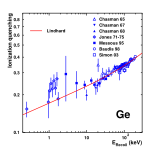
\includegraphics[scale=0.5]{Figures/Electrodes/ge_quenching.pdf}
\caption{Lindhard model of the ionization quenching factor in germanium (in red). Experimental results of direct measurements of the quenching factor from multiples experiments are displayed in blue.}
\label{fig:ge-quenching}
\end{figure}

% number of pairs
Immediately following the ionization process, electrons can be excited with energies much greater than the germanium band gap energy $E_g$. However, such electrons relaxes by phonon emission and creation of new electron-hole pairs. After the relaxation, we can consider that their is in the Ge crystal a number of pairs $N_p$:
\begin{equation}
\label{eq:number-pairs}
N_p = \frac{E_{Ion.}}{\epsilon_{e^--h^+}} =  Q \cdot \frac{E_R}{\epsilon_{e^--h^+}}
\end{equation}
with $\epsilon_{e^--h^+}$ the average energy of the relaxed electron-pairs. This equation demonstrates the key property of the semiconducting Ge crystal: the number of pairs $N_p$ is linked to the recoil energy $E_R$. Thus, its measurement yields an estimation of the recoil energy.

% presentation of the band conduction figure to explanation of lattice directions
This estimation requires to know the average energy of the pairs $\epsilon_{e^--h^+}$. A naive approach is to consider the band gap of the germanium $E_g$. It can be extracted from the electronic band structure of the germanium displayed in the figure \ref{fig:ge-band-structure}. The valence and conduction bands are plotted in the energy versus momentum space. The Germanium crystal possesses diamond cubic lattices. These repeating spacial pattern affects the electrons so that an available electronic states is defined by its energy and its momentum in respect to the crystal lattice. The momentum space is expressed using the Miller indices used to define the directions in the Ge crystal lattice.

\begin{figure}
\centering
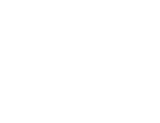
\includegraphics[scale=0.66]{Figures/Electrodes/germanium_conduction_bands.pdf}
\caption{Electronic band structure of the Germanium in the energy versus momentum space. Below the origin are the valence bands, above are the conduction bands. The minimum energy gap $E_g = \SI{0.67}{\eV}$ is set between the lowest-energy excited states in the valence bands at $\vec{k} \in \textsf{<000>}$ and conduction bands at $\vec{k} \in \textsf{<111>}$.}
\label{fig:ge-band-structure}
\end{figure}

% presentaion of the band conduction structure
In the figure \ref{fig:ge-band-structure}, the valence bands are situated below the origin while the conduction bands are above the origin. The minimal band gap $E_g = \SI{0.67}{\eV}$ of the germanium is derived from the lowest-energy states of excited carriers. Excited electrons, carrying a negative charge $-e$ are promoted to the conduction bands while the holes, carrying a positive charge $+e$, are created in the valence bands. The maximum of the valence bands corresponds to the <000> directions signifying a null momentum. The minimum of the conduction bands is obtained along the <111> directions. Excited electrons and holes have different momenta. As such, the germanium gap is defined as indirect: the transition of an electron to an excited state of the conduction band necessitate the transfer of a momentum $\vec{k}$ in addition to the gap energy $E_g$. This momentum transfer, present at the creation of the electron-hole pair and at for its recombination, is carried away by a third party which is a phonon in the germanium crystal. As a consequence, the average energy $\epsilon_{e^--h^+}$ contained in an electron-hole pair is greater than the germanium gap band of $E_g$ as it also takes into account the energy of the phonon of momentum $\vec{k} \in \textsf{<111>}$ associated with the pair. The average energy of an electron-hole pair in germanium is measured:
\begin{equation}
\label{eq:energy-pair}
\epsilon_{e^--h^+} = \SI{2.96}{\eV \per \textsf{pair}}
\end{equation} 
The relation \ref{eq:number-pairs} between the number of pairs $N_p$ and recoil energy $E_R$ is now applicable in the germanium.

% Number of electron-pairs created by a recoil
The number of created pairs $N_p$ is subject to fluctuation and thus impose itself as an intrinsic limit to the resolution of the ionization channel. The number of pairs $N_p$ should be expected to follow a Poisson distribution of standard deviation $\sigma(N_p) = \sqrt{N_p}$. However, experiments observed these fluctuations to be lower than expected . This can be explained by a correlation of the relaxation process of the phonons and electron-hole pairs. The empirical standard deviation is expressed as:
% paper [ref 85 quentin]
\begin{equation}
\sigma(N_p)
=
\sqrt{F \cdot N_p}
=
\sqrt{F \frac{Q \cdot E_R}{\epsilon_{e^--h^+}}}
\end{equation}
with an introduced Fano factor $F$ of about $0.1$ for the germanium. Considering the current range of ionization channel resolution, the fluctuation of the number of pairs created by ionization could be limiting with $\sigma(N_p) \approx \SI{300}{\kilo\eV}$ which could be obtained for electronic recoil energies greater than \SI{300}{\kilo\eV}. As we are interested in the lowest energy range and the experiments presented in this work use calibration peaks of energy in the order of $\mathcal{O}(\SI{10}{\kilo\eV}$, the impact of these fluctuation are negligible. This is especially true considering other effects with adverse impact on the ionization resolution such as the electronic noise of the electronic readout and incomplete charge collection.

% Impurities in germanium
The semi-conducting properties of a germanium crystal heavily depends on the impurities affecting it.
These impurities creates intermediary energy steps in the semi-conducting germanium band gap accessible to electric charges (as seen in figure \ref{fig:ge-band-structure}). The presence of these intermediate energy states  has several consequences on the ionization channel. It reduces the energy necessary to create an electron-hole pair, thus creating additional noise and biasing for the ionization channel. Then, it creates a trapping phenomenon which prevent electric charge carriers from reaching the electrodes. With trapped charges in the crystal, a counter electric field slowly generates, reducing the sensitivity of the electrodes. Finally, these impurities lower the global resistivity of the germanium crystal and increase the leakage current.
The semi-conducting germanium use as absorber thus should contain the lowest amount of impurities in order to have a detector with good performances.
%The study of the trapping in EDELWEISS detector and the impact of impurities is presenting in [ref quentin 80].
We define $N_a$ and $N_d$ as the number of acceptor and donor impurities respectively. We  can have access (how?) to the absolute difference of this quantities $|N_a - N_d|$ which determine the number of available charge carriers.
As a result, the EDELWEISS and RICOCHET experiment use High-Purity Germanium (HPGe) with a low impurity concentration:
\begin{equation}
10^{9} < |N_a - N_d| < 10^{10} \quad \textsf{in \si{\textsf{atoms}\per\cm^{3}}}
\end{equation}
which corresponds to less than one impurity atom for \num{e12} germanium atoms. As reference, a common germanium crystal possesses a concentration of about \SI{e13}{\textsf{atoms}\per \cm^{-3}}.  With this material, low leakage currents of few \si{\pico\ampere} can be achieved for the usual operating electric field range of a \si{\volt\per\cm}.


\subsection{Electric Charge Drifting in Crystal}
\label{par:charge-drifting}
%{\color{red} Alex B. biblio here. Also explainin trapping, charge collection.}

%% useless blabla
%The study of charge migration in EDELWEISS germanium crystal is presentend in [ref Emeline 82] taking into account the crystallographic structure of the germanium crystal. In this study, Alex.B simulates numerically the drifting of eletrons and holes in a 200g FID Edelweiss detector with bulk interaction of gamma-rays of energy 348keV. The charge trajectories are presented in the figure \ref{fig:charge-drifting}.
% He also follows the generation of the voltage signal on the electrodes. This is consistent with Ramo field theory which will be described later.

% Drifting simulation
The charge collection define the drift of the electric charge in the crystal under the influence of an electric field $\bm{E}$. The objective of this drift is for the charge to reach electrodes on the surface of the germanium crystal leading to a voltage signal measurable with an electronic readout. In this work, the magnitude of the electric field is of the order $\mathcal{\SI{1}{\volt\per\cm}}$. 

Following a recoil at a position $\vec{r}$ in the crystal, a high number $N_p$ of electron-holes pairs are created in the immediate vicinity of $\vec{r}$. This vicinity can be considered as a sphere of radius in the range of $\mathcal{O}(\SI{1}{\micro\m})$ in which the electric charges are evenly distributed due to an initial diffusion of the charges. From these initial positions, the electric charges propagate in the crystal under the influence of the electric field $\bm{E}$ and slightly by the presence of neighboring exited charges of same charges. 

The equations of motion of a single charge depends on the band structure of the germanium. As explained described earlier with the band structure of the germanium in figure \ref{fig:ge-band-structure}, the excited state of the electrons and holes are associated with momentum directions. On the one hand, the holes with $\vec{k} \in \textsf{<000>}$ presents an isotropic behavior in the crystal lattice as no momentum are to their excited state. They are thus free to propagate along the electric field lines. On the other hand, the excited states of the electrons are constrained with a momentum $\vec{k} \in \textsf{<111>}$. As such, the electrons show a strongly anistropic propagation in the crystal.

At low field strength, inferior to \SI{10}{\volt\per\cm}, the electrons are moving along the <111> valleys in the crystal. In practice, the direction of the electric field $\vec{E}$ corresponds to the vertical axis $\hat{z}$ of the cylindrical crystal which is along the <100> lattice directions. As such, the trajectories of the electrons are oblique forming a \SI{33}{\degree} with the vertical axis towards the higher electric potentials.
As high field strength, superior to \SI{10}{\volt\per\cm}, the probability of electrons scattering in the crystal and switching in another <111> valley is heightened. These inter-valley scattering are so common that the macroscopic trajectory of the electrons corresponds to the electric field lines. This behavior is observable in the vicinity of the FID electrodes where the electric field is increased due to the electric point effect.

% presentation of the oblique propagation figure
The figure \ref{fig:oblique-propagation} displays the simulated trajectories of electrons and holes drifting inside the semi-conducting Ge crystal of a \SI{200}{\g} EDELWEISS FID detector under the influence of an electric field. The holes drifts along the electric field lines and draw in red directs trajectories to the bottom collecting electrode. The electrons propagates towards the top collecting electrode following oblique trajectories in blue in the <111> directions. The charge drift last a few microseconds corresponding to a speed of the carriers in the order of $\mathcal{O}(\SI{1}{\cm\per\micro\s})$.

\begin{figure}
\centering
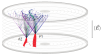
\includegraphics[scale=1]{Figures/Electrodes/transversal_trajectories.pdf}
\caption{Simulation of the drift of the electron-hole pairs in a semi-conducting germanium crystal of an EDELWEISS FID detector. The red trajectories of the holes $h^+$ follow the electric field lines. The electrons $e^-$ show an oblique propagation in blue along the <111> crystal directions. The direction of the average electric field $\langle \vec{E} \rangle$ imposed in the crystal is indicated on the right.}
\label{fig:oblique-propagation}
\end{figure}

The transversal motion of the electrons in the Ge crystal is problematic for the charge collection. Whereas the trajectories of the holes are predicted from the electric field lines, the electrons deviates from expectations. A s such, there is more error on forecasting the position of the electrons at the end of their drift and the resulting signal induced on the electrodes. 

% Trapping processes
Several processes can lead to an incomplete charge collection. An incomplete collection means the number of electron-hole pairs measured is lower than the actual number of pair created by a recoil. This happens when an electric charge does not reach its associated collecting electrode. This four phenomenon are: the bulk trapping, the surface trapping, the surface trapping, the crystal neutralization and the recoils under the electrodes.

% Bulk trapping
The bulk trapping corresponds to electric charge getting stuck in the crystal due to intermediate energy state induced by impurities in the crystal. This trapping is countered with the use High Purity Germanium. The amount of charge lost is proportional to the initial number created by the ionization process. As such, assuming a constant rate of bulk trapping, the sensitivity of the ionization channel is lowered but the measurement of the ionization energy $E_{Ion.}$ is feasible. In this work, the bulk trapping rate is estimated to \SI{2}{\percent} at a standard magnitude of \SI{2}{\volt\per\cm}. The bulk trapping rate depends on the electric field magnitude: while low magnitude $\mathcal{O}(\SI{0.1}{\volt\per\cm})$ boasts a high rate of bulk trapping, the application of a high electric field $\mathcal{O}(\SI{10}{\volt\per\cm})$ drastically reduces this rate.

% surface trapping
The surface trapping is happening when electric charges reach the bare surface of the Ge crystal. As opposed to the interior of the crystal with a controlled electronic band structure due to the repeating lattice, the germanium lattice stops on the surface creating irregularities in the band structure due to edge effects. These surface irregularities easily trap in place the electrons or holes. As such any charge reaching a surface is considered to have been surface trapped. This effect can be avoided for the holes: the detector are designed as to avoid electric field lines leaving the crystal. However, this counter has mitigated efficiency for the electrons due to their oblique propagation.

% crystal neutralization
The crystal neutralization refers to the progressive weakening of the electric field in the Ge crystal. All the electric charges trapped in the crystal produce a counter electric field. Depending on the crystal crystallography and the design of the electrodes, the electric field can lose in magnitude or can be warped, effectively becoming neutralized. This neutralization further boost the bulk trapping rate and can lead to unexpected surface trapping.
This phenomenon gains in intensity with the trapping rate, the event rate and the operation time of the detector. It usually becomes noticeable within hours to days. The crystal neutralization is countered by a "regeneration" procedure. It consists in grounding all the electrodes of the detector and submitting it to an intense event rate in order to shake up the trapped charges. These events are generally originating from a LED or a radioactive source. Stuck charges are excited out of their traps and recombines under the influence of their own counter electric field. As the detector is not available for data taking in this condition, the period between two regeneration procedures should be empirically adjusted to the measured charge accumulation while not too frequent to avoid supplementary dead times. For the above-ground operation at IP2I, a regeneration is realized ever two days. A radioactive cesium source of high activity of about \SI{4e10}{\becquerel} is placed on the outside of the closed cryostat at about \SI{20}{\cm} from the detector load.

%While a maintenance shakes up the majority of the trapped electric charges, a small fraction is not affected and participates to build up the counter field. These remaining charges are deeply trapped and need for a stronger perturbation to be freed. The detector is therefore periodically submitted to a procedure called "regeneration" aiming at a full reset of any passive electric field in the germanium crystal. With the electrodes being grounded, an intense gamma-ray radioactive source irradiates the detector. The high frequency of high energy recoils produces ionization in the whole crystal which eventually neutralize the accumulated space charges. 
%While the majority of the electric charges produces by the ionization process are collected by the electrodes, some become trapped in the crystal (impurities) or on the surfaces of the crystal. These trapped charges are slowly accumulating and creating a counter electric field in the absorber. This results in a lower electric field perceived in the bulk of the detector which hampers a correct charge collection and decreases the sensitivity of the electrodes.


% Recoils under the electrodes
The recoils under the electrodes are rare occurrences when the electron-hole pairs are created at a few tens of \si{\micro\m} under the aluminium electrodes deposited on the germanium surface. These surfaces of the germanium crystal are specially prepared as to allow the correct deposition of the aluminium. This result in a metallic behavior of the germanium in the vicinity of the electrodes, thus creating a extension of the electrode in the crystal. With virtually no energy gap, charges created in these regions immediately recombines and do not drift under the influence of the electric field. This phenomenon is countered by processing the surface under the electrodes and creating a layer of amorphous layer of high band gap. This amorphous layer separates the crystal from the metallic layer and prevent the undesired recombinations.


\subsection{Electrode Deposition on the Germanium Crystal Surface}

%*Stefanos biblio here.*
%% blabla
%The aluminium deposition is carried out by the research group at CSNSM at Orsay.
% The deposition processes are still being improved.

The electrodes of the ionization channel consists in aluminium deposits on the surface of the germanium crystal. The germanium crystal is placed in a vacuum chamber where its surface can be processed with beams of vaporized atoms. These atoms are radicals, atoms with unpaired valence electrons, with high chemical reactivity. As such, these radicals reacts with any material in place. This technology is use in the creation of thin layers and for the precise alteration of the germanium surface. A solid mask can be set between the beam source and the crystal in order to shape the altered surface. In the case of the cylindrical crystal of this work, the top and bottom planar faces as well as the lateral surface can be faced towards the beam source. The crystal is usually rotated around its vertical axis to assure the homogeneity of the aluminium deposition. 

% amorphous layer
Before depositing aluminium, it is necessary to prepare the germanium surface meant to host the aluminium layer. The preparation step is the creation of the amorphous layer meant to host the aluminium deposits. The germanium surface is locally altered with a beam of vaporized hydrogen atoms to form a layer about \SI{80}{\nm} deep of hydrogenated germanium. As mentioned is the previous paragraph, this compound is highly resistive preventing an early recombination of the electron-hole pairs. Another advantage of this layer it reduces leakage current between the electrodes through the surface of the germanium.

% aluminium layer
The next step is the actual deposition of the aluminium using a beam of vaporized aluminium atoms. An aluminium layer is estimated to be about \SI{50}{\nano\m}. A layer with a continuous shape is called an aluminium deposit. For cylindrical germanium crystal, we call "full planar electrode" an aluminium deposit covering the entirety of the planar surface.
% Shaping the deposits
Two techniques are used to form shapes with the deposits.
The most straightforward method is the evaporation of aluminium with a mask. This technique is precise and quick but is limited to simple pattern respecting the cylindrical symmetry of the crystal. The most remarkable deposit shape in use for the FID detectors of the EDELWEISS-III experiment is the concentric circular rings. The mask  consists in several curved slits which allow the passage of vaporized aluminium. By rotating the mask during the process, the aluminium is deposited in a ring pattern on the germanium. The electrodes of the design FID38 would likely be produced in the same way.
The other technique is called the photolitography. First, the whole surface of the crystal is covered with a layer of aluminium. Then, the aluminium is coated with a chemically-protective wax. The negative of the electrode pattern is carved in the wax coating with the use of lasers, hence the name photolitography. Once done, the germanium crystal face is immersed in a chemical solution reactive with aluminium. Only the aluminium protected by the wax (patterned as the desired electrode design) is left on the surface. Finally, the wax coating is removed with an other chemical. The process has some drawbacks compared to the use of mask: it is longer and can be less precise due to the chemical attack of the aluminium. However, this method can produced any pattern desired such as  square grids and holes useful for hosting the NTD thermal sensor on the germanium surface.
An inevitable constraints on the shape of the aluminium deposits is the minimum width of thin deposits (such as rings) of about \SI{50}{\micro\m}.

% cabling
We now describe how these thin aluminium deposits can be cabled to the electronics and considered as electrodes.
The fragility of the germanium and the shallow aluminium layers motivate the use of wire-bonding as cabling technique. It consists in soldering \SI{25}{\micro\meter} thin metal wires on the aluminium deposits. Wedge bonding is used to solder the metal to the aluminium using ultrasonic power and force the bonding. Two metal are used for the wire-bonding: aluminium and gold. Both can conduct the electric current however the aluminium is superconducting at cryogenic temperature making it acts as a heat insulator. As such, aluminium wires are commonly used and gold wires are reserved for the creation of a controlled thermal leak as discussed in the chapter \ref{ChapterEthem}.

In the case of simple electrodes like the PL38 design or the RED80 detector, several wires link the top (and bottom) electrodes to a conductive pad on the detector copper chassis. The conductive pad is then cabled to the ionization electronics.
With more complex design like the FID38 design or the REDN1 detector, wires are used to connect different aluminium deposits, essentially imposing the same electric potential is those. With two wire bridges, it is possible to create interleaved electrodes with a biasing scheme based on the co-planar grid technique for event localisation used in the FID detectors of the EDELWEISS-III experiment. This biasing scheme is later described in this chapter for the FID38 design.
%[ref emeline 86]

\subsection{Shockley–Ramo Theorem}
\label{par:shockley-ramo}

%%% useless blabla
%[ref quentin 100 101 102]
%\begin{equation}
%\label{eq:ramo-theorem-integrated}
%Q_X = - q \Phi_X(\vec{r})
%\end{equation}

The ionization channel is based on the induction of a voltage signal $\Delta V$ on the electrodes  of capacitance $C$ by collecting drifting charges $\Delta Q$. A naive but false explanation to this signal generation is to consider that the charge $\Delta Q$ is entirely deposited instantly when the charges reach the electrode. The correct explanation is to consider the current $i$ induced on the electrode starting from the moment the electrons and holes drift in the crystal. This signal induction is theorized with the Shockley-Ramo theorem which states that the current $I_X$ induced on a given electrode, labeled $X$, due to the motion of a charge in an given electric field $\vec{E}$ created by multiples electrodes, is given by:
\begin{equation}
I_X = q \cdot \left( \vec{E}_X \cdot \vec{v} \right)
\end{equation}
%= q \cdot E_v \cdot \| \vec{v} \|
where $q$ is the charge of the particle, $\vec{v}$ its velocity and $\vec{E}_X$ the "weighting electric field" associated to the electrode $X$. This weighting field $\vec{E}_X$ is virtual and differs from the actual electric field $\vec{E}$ in the crystal. The weighting electric field $\vec{E}_X$ associated to the electrode $X$ corresponds to the electric fields in the crystal with all free charges removed, the given electrode $X$ raised to unit potential $V_X = \SI{1}{\volt}$, and all other conductors grounded. This theorem ensues from the Gauss theorem.
An interpretation of the Shockley-Ramo theorem is that a charge moving in the vicinity of an electrode induces an instantaneous electric current by affecting the electrostatic field lines ending on the electrode.
This theorem can be integrated to access the instantaneous induced charge $Q_X$ on the given electrode $X$. In the case of a drifting charge $q$ of initial position $\vec{r_{q,i}}$ and final position $\vec{r_{q,f}}$, the total integrated charge induced on the electrode $X$ is:
\begin{equation}
Q_X = q \left( \Phi_X (\vec{r_{q,f}}) - \Phi_X (\vec{r_{q,i}}) \right)
\end{equation}
The term $\Phi_X(\vec{r})$ is called the "weighting potential" of the electrode $X$ at the position $\vec{r}$. It is derived from the weighting electric field associated to the electrode $X$ using the usual formula:
\begin{equation}
\vec{E}_X (\vec{r}) = - \left. \overrightarrow{\mathrm{grad}} \left(  \Phi_X \right)  \right|_{\vec{r}}
\end{equation}
By definition of the weighting electric field $\vec{E}_X$, the weighting potential $\phi_X$ takes its values from the $[0,1]$ interval. The weighting potential field associated with a point-like electrode $X$ situated at a position $\vec{r}_X$ in an empty space is $\Phi_X$ with the following properties:
\begin{equation}
\label{eq:ramo-particle}
\begin{cases}
\lim_{||\vec{r} - \vec{r}_X|| \to \infty} \Phi_X(\vec{r}) = 0 \\
\lim_{||\vec{r} - \vec{r}_X|| \to 0} \Phi_X(\vec{r}) = 1
\end{cases}
\end{equation}
This property is generalized to any other shape of electrode at any point on its surface.

The Shockley-Ramo theorem benefits from the superposition theorem such that it is possible to express the signal induced on the electrode $X$ by charges drifting after the creation of a number $N_p$ of electron-hole pairs:
\begin{equation}
\begin{split}
Q_X &= \sum_{n=1}^{N_p} \left( Q_X^n(e^-) + Q_X^n(h^+) \right) \\
&= \sum_{n=1}^{N_p} -e \left( \Phi_X (\vec{r}_{e^-,f}^n) - \Phi_X^n (\vec{r}_{e^-,i}^n) \right) +e \left( \Phi_X^n (\vec{r}_{h^+,f}^n) - \Phi_X (\vec{r}_{h^+,i}^n) \right)
\end{split}
\end{equation}
where exponent $n$ expresses the association with the carrier of the $n$-th pair.
When considering the drifting of a single electron-hole pair, the initial position is the same for both charges with:
\begin{equation}
\forall n, \quad \Phi_X(\vec{r}_{e^-,i}^n) = \Phi_X (\vec{r}_{h,i}^n)
\end{equation}
The charge induced induced by the drifting of $N_p$ electron-hole pairs is simplified to:
\begin{equation}
\label{eq:ramo-induced-charge}
Q_X = e \sum_{n=1}^{N_p} \left( \Phi_X (\vec{r}_{e,f}^n) - \Phi_X (\vec{r}_{h,f}^n) \right)
\end{equation}
An important remark is that the induced signal solely depends on the weighted potential of the final position of the charges. As mentioned in the previous paragraph, the charge trapping process induces a loss in signal. Indeed, they prevent the drifting charge from reaching an electrode where its contribution to the induced charge is maximal.

%While the vast majority of charges ends up collected in the electrodes and participate with a weighted potential of $\pm 1$, some charges are trapped and so participate to the signal with the weighted potential corresponding to the position of the trap, which reduces the induced signal.

The total weighting potential (TWP)  field is defined as the sum of the weighting potentials associated with all the $N$ electrodes $X_k$ composing the ionization channel:
\begin{equation}
\label{eq:twp}
Q_T (\vec{r}) = \sum_k^N Q_{X_k} (\vec{r})
\end{equation}

If the electrodes of the detector form a perfect Faraday cage, all the field lines end on the electrodes and none is leaving the crystal. As a result, when considering a unique charge $q$ in the crystal, the total weighted potential $Q_T$ is equal to the charge at any moment of the drift, $Q_T = q$. When considering $N_p$ electron-holes pairs, the Faraday cage imposes the charge conservation on the total weighting potential such that $Q_T = 0$.

In the later paragraph \ref{par:weighting-potential}, we further the discussion on the weighting potentials using the electrostatic simulation of the PL38 and FID38 detector designs as illustration. Also, the Shockley-Ramo theorem is used to model the signal generation for these detectors.

%Should I include the study of the trapping by Quentin ? Some studies [103 and 104 quentin ref] were done on the dependance of the electric charge  trapping in germanium crystals. Electrons are more prone to be trapped than hole. According ti Quentin, 10 to 20\% of the carriers are trapped (?). He then calculates the signal induced with trapping and also the effect of trapping as a function of the trap localization. And the impact of trapping on the heat channel.


\subsection{Luke-Neganov Effect}
\label{par:luke-neganov}

%%% useless blabla
% [ref 63 emeline]

% reserve
The Luke-Neganov effect has major impacts on the heat channel and the efficiency of the discrimination provided by the combination of the heat and ionization channels. While this effect depends on the electric field applied by the electrodes, it has no influence on the charge collection or the signal generation on the electrodes of the detectors.  

% presentation of the effect
When electric charges drift under the influence of the applied electric field $\vec{E}$ in the germanium crystal, they create phonons. This process is called the Luke-Neganov effect. This phenomenon happening in semiconductors is analogous to the well-known Joule Effect present in conductors. The phonons created draw their energies from the work $W$ of the electric field $\vec{E}$ on the drifting charge $q$ such that: 
\begin{equation}
W
=
q \int_{ \vec{r}_{q,i} }^{ \vec{r}_{q,f} } \vec{E} \ \mathrm{d}\vec{r}_q
=
q \int_{ \vec{r}_{q,i} }^{ \vec{r}_{q,f} } \frac{\partial V}{\partial \vec{r}} d\vec{r}
=
q \cdot \left( V(\vec{r}_{q,f}) - V(\vec{r}_{q,i}) \right)
\end{equation}
%As discussed in the chapter \ref{ChapterEthem}, as the phonons thermalize in the crystal, their momentum is converted into thermal energy adding to the initial heat energy of the recoil. 

In the case of a recoil producing $N_p$ electron-hole pairs, the work provided by the electric field going into the phonon bath and eventually the heat channel is defined as the Luke-Neganov energy $E_{NL}$ also known as the Luke-Neganov boost as it is added to the initial heat energy of the recoil. It is expressed as:
\begin{equation}
E_{NL}
=
e \sum_{n}^{N_p} \cdot \left( V(\vec{r}_{h^+,f}^n) - V(\vec{r}_{q,i}^n) \right)
+ 
(- e) \sum_{n}^{N_p} \cdot \left( V(\vec{r}_{e^-,f}^n) - V(\vec{r}_{e^-,i}^n) \right)
\end{equation}
Similarly to the application of the Shockley-Ramo theorem to a recoil, the electron and the hole of a same pair have the same initial position such that $V(\vec{r}_{q,i}^n) = V(\vec{r}_{e^-,i}^n$. As such, the expression of the Luke-Neganov energy simplifies to:
\begin{equation}
E_{NL}
=
e \sum_{i=0}^{N_p} \left( V(\vec{r}_{h^+,f}^n) - V(\vec{r}_{e^-,f}^n) \right)
\end{equation}
It appears that $E_{NL}$ depends solely on the electric potential $V$ in the crystal at the final positions of the electron $\vec{r}_{e^-,f}^n$ and the hole $\vec{r}_{h^-,f}^n$.


%are created and eventually participate to the heat signal.
%The drifting electrons constantly dissipate their energy to the phonons bath. As the electrons stay in motion and are eventually collected by the electrodes, the electric field must provide a work $W$ compensating the energy loss going into the heat channel.
%\begin{align}
%W &= q_{e^{-}} \int_{ \vec{r_i} }^{ \vec{r_{e,f}} } \vec{E} d\vec{r} - q_{h^{+}} \int_{ \vec{r_i} }^{ \vec{r_{h,f}} } \vec{E} d\vec{r} \\
%&=  -e \int_{ \vec{r_i} }^{ \vec{r_{e,f}} } \frac{\partial V}{\partial \vec{r}} d\vec{r} + e \int_{ \vec{r_i} }^{ \vec{r_{h,f}} } \frac{\partial V}{\partial \vec{r}} d\vec{r} \\
%&= e \left( V(\vec{r_{h,f}}) - V(\vec{r_{e,f}}) \right)
%\end{align}
%where $q_{e^{-}} = e = - q_{h^{+}} $ represent the electric charges and $\vec{r_{i,f}}$ is the final position of the electric charge $i \in \{e^{-}, h^{+}\}$. 

A useful, and mostly accurate, assumption is to consider the complete charge collection: all the charges end their drift by reaching the electrodes polarized at potentials $V_+$ and $V_-$. The Luke-Neganov boost is further simplified to:
\begin{equation}
E_{NL} = N_p \cdot e \cdot (V_+ - V_-) = N_p \cdot e \cdot \Delta V
\end{equation}
The Luke-Neganov effect is proportional to the number of pairs $N_p$ created in the ionization process and the voltage bias $\Delta V$ of the detector. Using the equation \ref{eq:number-pairs}, we can express the boost as a function of the recoil energy $E_R$ and the quenching factor $Q$:
\begin{equation}
E_{Luke-Neganov} = \frac{E_{Ion.}}{\epsilon_{e^--h^+}} \cdot e \Delta V = Q \frac{E_R}{\epsilon_{e^--h^+}} \cdot e \Delta V
\end{equation}
Although they deposit the same recoil energy $E_R$, an electronic recoil benefits more than a nuclear recoil from the Luke-Neganov boost according to the hierarchy of their quenching factor $Q_{ER} > Q_{NR}$. 
A useful simplification is to consider that $e / \epsilon_{e^--h^+} = 1/2.97\ \si{\per\volt}$,  and to have a final expression of the Luke-Neganov boost as:
\begin{equation}
\label{eq:nl-boost}
E_{NL} = Q \cdot E_R \cdot \frac{\Delta V}{2.97}
\end{equation}

It is essential to take into account the Luke-Neganov energy when reconstructing the recoil energy $E_R$ from the measured heat energy $E_{heat}$ given that:
\begin{equation}
E_{heat} = E_R + E_{NL} = E_R \cdot \left( 1 + Q \frac{\Delta V}{2.97} \right)
\end{equation}

The Luke-Neganov effect is a very interesting strategy to enhance the sensitivity of the heat channel. However, this heat channel boost is applied at the expanse of the discrimination ability of the detectors thanks to the double heat-ionization energy measurement. When operating the detector with a very high voltage bias $\mathcal{O}(\SI{10}{\volt})$, the Luke-Neganov boost dominates in the expression of the measured heat energy $E_{heat}$:
\begin{equation}
\Delta V \gg \frac{2.97}{Q}
\quad \Rightarrow \quad
E_{heat} \approx E_{NL} \propto E_{Ion.}
\end{equation}
The heat energy becomes equals to the ionization energy ignoring the multiplicative factor. As such, it becomes impossible to distinguish discriminate the electronic recoils from the nuclear recoils as their signature in the same. In fact, this observation can be further at any voltage bias: the existence of the Luke-Neganov effect diminishes the discrimination power of the ER and NR events. As this feature is essential for the correct operation of the the detector and to reach their scientific goals, the Luke-Neganov effect should be kept minimal by aiming at low voltage bias in the detector design.

%This is very important to keep in mind when reconstructing the recoil energy $E_R$ from the measured heat energy $E_{heat}$ as it is a function of the deposited recoil energy $E_R$ and the recoil type $j$:
%\begin{align}
%E_{heat} (E_R, j ) &= E_{R} + E_{Luke-Neganov} ( E_R, j) \\
%&= E_R \left( 1 + Q^j(E_R) \frac{\Delta V}{3} \right)
%\end{align}


\subsection{Polarization and Readout Electronics of the Ionization Channel}
%\subsection{DAQ and electronics for ionization}
\label{par:electronics-ionization}

%%% useless mumbojumbo
%As each electrode is considered as a terminal of a capacitor $C_{electrode}$, the measured voltage is:
%\begin{equation}
%\Delta U = \frac{\Delta Q}{C_{electrode}}
%\end{equation}
%with $Q$ the drifting charge seen by the electrode.

% Introduction
The electronics associated with the ionization channel has two functions: the signal readout and the polarization of the electrodes. As usual, the electronics are separated in two stages: the cold electronic inside the cryostat, before any signal amplification, and the hot electronics outside of the cryostat transferring the amplified signal. This paragraph focuses on the cold electronics which has major influence on the resolution of the ionization channel and the operation of the ionization channel. The readout and the polarization of all the electrodes of a detector are driven by a single computer. However, we can  consider that each electrode is equipped with an independent cold electronic line.

% Cricuit presentation
Figure \ref{fig:electronics-scheme} shows two electric circuits of the electronic line of a single electrode of a detector. The circuit on the left represents the current electronics of the IP2I cryostat used to realize all the ionization measurements presented in this work. It uses Junction Field Effect Transistor (JFET). On the right is a representation of a High Electron Mobility Transistor (HEMT) based electronics in development for building the RICOCHET experiment and enhancing the performance of the EDELWEISS experiment.

\begin{figure}
\centering
\includegraphics[width=0.48\textwidth]{Figures/Electrodes/electronic_ion_ip2i.png}
\includegraphics[width=0.48\textwidth]{Figures/Electrodes/electronic_ion_hemt.png}
\caption{Scheme of a cold electronics line for the ionization channel currently used at IP2I (left) and in development with HEMT technology (right). The electronics line assures the polarization of the electrode and the signal readout. One of the main difference is the floating state of the current electronic (heaviside signal) versus the polarization resistance of the HEMT (decaying exponential signal).}
\label{fig:electronics-scheme}
\end{figure}

The readout of the JFET-based and HEMT-based electronics lines measure the same physical quantity: the electric potential of the electrode. The JFET and HEMT are used to readout and amplify the voltage signal. This method can differ from other experiments equipped reading the current induced by the drifting charge on a feedback capacitance with a charge amplifier. Compared to a charge amplifier, a voltage amplifier does not involve any resistor in the amplification scheme, resulting a lower electronic noise. However, the use of a voltage amplifier is only possible with low leakage current lower than \SI{0.1}{\femto\ampere}.
One should note that the amplifying transistor situated at the end of the electronic line are separated from the electrode, represented by the capacitance $C_d$, by a coupling capacitor of high value $C_c \sim \mathcal{O}(\SI{1}{\nano\farad})$. This ensures that the electrical charges of the electrodes are not going into the readout electronics.

% (good for EDELWEISS, but is this possible for RICOCHET with operation on surface).
The electronics lines are designed to assure its functions while keeping the electronics noise as low as possible. Once the signal is amplified, it is transmitted to the acquisition computer through the hot electronics without adding additional noise.

There are several differences between the current JFET-based and the future HEMT-based electronics.
% Diff JFET and HEMT
The main change concerns the technology of the voltage amplifier. The JFET are operated at a low temperature of \SI{100}{\kelvin} inside the cryostat. At the time of design for the EDW-III experiment, this technology offered the best performances. Nowadays, recent breakthrough in the electronics field adapts the HEMT technology to the constraints of the EDELWEISS and RICOCHET experiments. With a HEMT are operated at the lower cryogenic temperature of \SI{1}{\kelvin}, the thermal noise of the electronic components is reduced leading to an overall reduced noise injection in the amplification scheme.

% Polarization
The other main differences resides in the polarization of the electrodes. The polarization is the process of fixing the electric potential of an electrode.
In the current JFET-based electronics, this process is assured by a mechanical relay (represented by the polarization switch on the figure \ref{fig:electronics-scheme}) linking the electrode to a constant voltage source. By switching on, the electrode, acting as the plate of a capacitor, is accumulating charges and eventually reaches the aimed potential. By switching off, the electrode keeps the accumulating charge and its now fixed electric potential. Due to the relay opening the circuit, the constant voltage source cannot induce any electronic noise on the electrode.
The downside of this method is the progressive neutralization of the polarization as the electrode collects charges. Moreover, in the case of the RICOCHET experiment with surface operation of the bolometers, the event rate is high leading to a faster discharge.
% Maintenace procedure
The counter is to periodically switching on and off the relay in order to re-establish the wanted potential on the electrode. This procedure is called “maintenance”. In reality, a maintenance lasts one minute and consists in multiples relay switches and relay changeovers. During this one minute of maintenance, the detector is not available for data taking. This is enforced by the "maintenance cut" described in the paragraph \ref{par:maintenance-cut}. The frequency of maintenance is adapted to the condition of operation of the detector: too much maintenance induces unnecessary dead time while too few leads to a lower and uncontrolled voltage bias. For above ground operation at IP2I, the usual maintenance period is of about 30 minutes and should be empirically adjusted to the detector and the event rate.
% Continuous polarization
For the HEMT-based electronics, the polarization is continuously assured by a constant voltage source $eDAQ$ in series with a resistor of high impedance $R_{Polar.} = \SI{e10}{\ohm}$. While this method induced supplementary electronic noise, there is no more dead time and the maintenance procedure is not needed.

% Some numbers for the ionization readout
% sampling frequency and ionization signal shape
The ionization channel readout is sampled at an initial frequency of \SI{100}{\kilo\Hz}. This means the period of the  measurement points is \SI{10}{\micro\s} which is still greater than the estimated time span of an ionization signal of a few \si{\micro\s}. As a result, an ionization signal is recorded as an Heaviside function. No information can be obtained on the shape of the signal. The high readout sampling was historically chosen in EDELWEISS for the purpose of synchronizing an external detector vetoing incoming muons with a good timing resolution. The highly sampled ionization signal is then averaged in order to produce a signal of sampling frequency $f_s$. This sampling frequency is a parameter of the acquisition and can be set in the range $[200, 1000]\ \si{\Hz}$. This lower sampling records the information contained in the Heaviside-shaped ionization signal (its amplitude mainly) while being lightweight in term of disk space, which is essential considering the recording and processing resources at our disposal. The saved ionization signal of sampling frequency $f_s$ is composed of points whose values are averages of $\SI{100}{\kilo\Hz}/f_s$ points. In the end, the saved signal of an event of sampling frequency $f_s$ is therefore Heaviside-like function $H(t)$ with a varying value $H(t=0)$.

% Digitization
The ionization signal is readout as a digital signal which can take, by definition, a limited number of values. This readout range contains 64000 values which are sorted on the so-called readout dynamic range $[-32000, +32000]$ expressed in Analog-to-Digital Unit (ADU). For the ionization channel, the correspondence between ADU and Volt is \SI{67.4}{\nano\volt\per\textsf{ADU}}. As such, the dynamic range can records perturbation with a maximum amplitude of \SI{2.156}{\volt}. As a reference, the sensitivity of the ionization channel is about $\SI{60}{\textsf{ADU}\per\kilo\eV} \approx \SI{4}{\micro\volt\per\kilo\eV}$. A high event rate of low energy events or single high energy events can rapidly make the data stream fall out of this dynamic range, effectively saturating the acquisition electronics.
% Reset procedure
As to avoid this phenomenon and correct it, both electronics circuit features a feedback line. A procedure called “reset” consists in linking the input of the amplifying transistor to a null potential as to recenter the recorded signal on 0 ADU. The linking is assured in the feedback line with mechanical relays. Each reset induces an artifact signal on both the heat and ionization channel. While it can be easily discriminate from real events due to its shape, these artifact signals are discarded by applying the reset cut during the data analysis presented in the paragraph \ref{par:reset-cut}. As such, reset procedures creates dead times during which the detector is not available for data acquisition. Similarly to the maintenance period, the period of the reset is empirically adjusted to reach a balance between dead time and dynamic range saturation. The period of the resets is of a few seconds. In the case of surfaces operation at IP2I, the event rate is high and lot of charges are accumulated which needs for a shorter period than an underground operation.

%The ionization channel readout being based on the collection of electric charges, the renewal of the electric potential of the electrodes is necessary to maintain the voltage bias of the detector and to prevent the signal from leaving the readout range $[-32000, +32000]\ \textsf{ADU}$.


\subsection{Objective of the Electrodes Study}
\label{par:ionization-objective}

Three chapters of this work are dedicated to the study of the ionization channel and the electrodes design: this chapter \ref{ChapterElectrodes} introducing the theory and the electrostatic simulation of the ionization channel,  chapter \ref{ChapterElectrodesScan} scanning over the parameters of the electrostatics simulation, and the chapter \ref{ChapterElectrodesExperimental} comparing the electrostatics simulation to experimental results.

The main objective of these studies is to propose an electrode design for \SI{38}{\g} germanium crystals with optimal performances of the ionization channel. The performances of the ionization channel depends on several aspects: the energy resolution, the effective volume and the charge collection. As such, the study aims at drawing relation between the electrodes design and these aspects.

The energy resolution is roughly a signal-to-noise ratio. There is two ways to lower the energy resolution: increase the sensitivity to the signal or reducing the noise affecting the measure.
% Sensitvity
The sensitivity of the ionization channel is describe in a simplistic manner with the equation \ref{eq:capacitor-basic}. The voltage signal is inversely proportional to the capacitance of the electrodes. The modelization of the ionization channel is furthered in the later section \ref{sec:simulation-ionization} with a more accurate theorization of the signal generation, yet pointing towards a similar relation between sensitivity and electrode capacitance. As a starting point, we can model a simple and naive ionization channel as a parallel plate capacitor whose dielectric is the cylindrical germanium crystal. The associated capacitance without edge effects is:
\begin{equation}
\label{eq:parrallel-plate-capacitor}
C = \epsilon_0 \cdot \epsilon_r(Ge) \cdot \frac{A}{d}
=
8.854 \times 10^{-12} \times 16.3 \times \frac{\pi \cdot (15 \times 10^{-3})^2}{10 \times 10^{-3}}
=
\SI{10.20}{\pico\farad}
\end{equation}
with $\epsilon_0$ the electric constant and $\epsilon_r(Ge)$ the relative permittivity of the germanium. The area $A$ of the circular electrodes is imposed by the geometry of the germanium crystal of height $d=\SI{10}{\mm}$ and radius \SI{15}{\mm}. This capacitance of \SI{10}{\pico\farad} yielded by this naive modelization is set as the objective for the electrode design. 
% Noise
Regarding the noise affecting the ionization channel, it is for the moment dominated by the voltage and current noise induced by the JFET-based electronics. The intrinsic noise associated with the polarization process is negligible. As such, efforts are made to model the lower noise of the future HEMT-based electronics and optimizing the design of the ionization channel to reduce it further. With some early calculations, and considering the objective \SI{10}{\pico\farad} capacitance, an objective of \SI{10}{\eV} is set for the energy resolution of the ionization channel.

% Fiducial volume
The effective volume refers to the volume fraction of the germanium crystal in which the ionization energy of events is well reconstructed. This notion is developed later as the fiducial volume. Having a high fiducial fraction close to \SI{100}{\percent} ensures that the whole volume acts as a valid target for the particle interaction. As such the exposure of the detector is maximized and more statistics is collected. That is crucial to estimate the scientific goals and the time scale of the RICOCHET and EDELWEISS experiments. 

% Charge collection
The good charge collection is a broad concept that aims at having a predictable and reliable signal generation by the drifting charges drifting. Collection problems such as charge trapping can induced abnormal signatures increasing the noise in the energy reconstruction or, worse, emulating an inexistent dark matter or CENNS event. 

Lastly, this work is part of the research and development of detectors for two experiments. Event though their scientific goals are similar, the operating conditions are different resulting in different constraints on the detector design. A major difference affecting the electrode design is the high event rate associated with the above ground operation for the RICOCHET experiment compared to the low radioactive background of the underground EDELWEISS experiment. 

%2 Experiments : EDELWEISS and RICOCHET with different operating conditions (underground vs above ground operation, etc..)
%\begin{itemize}
%	\item EDELWEISS is limited by the radioactive background
%	\item RICOCHET is limited by the signal-over-noise ratio
%\end{itemize}


\section{Electrostatic Simulation of the Ionization Channel}
\label{sec:simulation-ionization}

In this section, the detector designs PL38 and FID38 are simulated using the Finite Element Method software COMSOL Multiphysics. The modelization of the ionization channel is illustrated with these electrostatics simulation. In particular, the relation between the electrode designs of PL38 and FID38 and their respective sensitivities and electronic noise is thoroughly theorized.

\subsection{Finite Element Method Applied to Electrostatics}

% Intro to Finite Element Method
The software COMSOL Multiphysics aims at simulating physics system based on the finite element method. 
The finite element method (FEM) is the most widely used method for solving problems of engineering in fields such as structural analysis, heat transfer, fluid flow, mass transport, and increasingly more. The domain which is of interest for this work in the resolution of electrostatics equations. In particular, the simulations of the PL38 and FID38 necessitate the extension "AC/DC" of COMSOL Multiphysics offering advanced features for the electromagnetic and electronic systems.
% Why use that
A cryogenic germanium detector represents a complex electrostatic system whose associated equations do not present easily accessible analytical solutions. The use of an FEM software is motivated by its ability to accurately represent a physical system with a complex geometry. It can takes into account multiples materials with each their own physical properties. The total solution can be easily represented with access to both global properties of the system and local effects. Additionally, such a software offers a readily operational framework for the geometry building, the mesh optimization and the equation resolution. With a relatively short learning period, this permitted to invest an extended period of time to the analysis of the results yielded by the simulation. 

% Method description
The FEM is a particular numerical method for solving the partial differential equations associated with a system in two or three space dimensions. 
% Discrtization
To solve a problem, the FEM subdivides the large system into smaller, simpler parts which are called finite elements. This space discretization is implemented by constructing a mesh of the object with a finite number of nodes, also called vertices. Multiples neighbors vertices forms a finite element. There are multiples geometries possible for a finite element. In this work, the meshes are combinations of lines, triangles and tetrahedrons. For the simulation of the PL38 and FID38 designs, the mesh parametrization is discussed and illustrated in the next paragraph \ref{par:mesh-parametrization}

% Equation resolution
% Each of finite element of the mesh serves as a domain for the numerical resolution of the equations.

Each finite element of the mesh is associated with a set of element equations. The element equations are simple equations that locally approximate the original complex equations of the larger whole system. In this work, these are the electrostatics equations satisfied by the electric potential field $V$. They are defined by the relation between electric potential and electric field $\vec{E}$:
\begin{equation}
\label{eq:potential-definition}
\vec{E} = - \nabla V
\end{equation}
and the Gauss law:
\begin{equation}
\label{eq:gauss-law}
\nabla \cdot \left( \epsilon_0 \epsilon_r \vec{E} \right) = \rho_f
\end{equation}
where $\rho_f$ is the volume density of free charge. The boundary conditions are first set by the interface condition:
\begin{equation}
\vec{n} \cdot \vec{E} = 0
\end{equation}
with $\vec{n}$ the normal vector at boundaries between materials. Then comes the electric potential fixed by the ground $GND$ and the electrodes $X_n$:
\begin{equation}
\begin{cases}
\forall \vec{r} \in \Sigma (GND): & \quad V(\vec{r}) = 0 \\
\forall n, \forall \vec{r} \in \Sigma ( X_n ): & \quad V(\vec{r}) = V_{X_n}
\end{cases}
\end{equation}
where $V_{X_n}$ is the fixed electric potential of the $n$-th electrode of the detector and $\Sigma$ designates a surface.

All these equations constitute a steady state problem, independent of the time, in which the original partial differential equations are approximated with a set of polynomial equations. The system is solved by a true solution function, here the electric potential field $V$ which is unknown. As such, this unknown true solution is approximated by the numeric solution $V_h$. This numeric solution is usually a piecewise function assembling linear approximation over all the finite element. 
% Figure presentation
The figure \ref{fig:fem-illustration} illustrates the approximation of a true solution by an approximate numeric solution $V_h$. On the left, a 1-Dimensional problem is solved. The numeric solution is a linear combinations of basis functions $\Psi_i$ such that
\begin{equation}
V_h (\vec{r}) = \sum_i V_i \cdot \Psi_i (\vec{r})
\end{equation}
where $V_i$ are the weights. The basis function $\Psi_i$ corresponds to a unitary triangular function centered on the position $x_i$ of the $i$-th node.
The result of the approximation is that all the partial differential terms are easily calculated. This choice of approximation applied to the equation \ref{eq:potential-definition} on the $i$-th node of the 1-D problem yields:
\begin{equation}
\vec{E} (x_i)
\approx
\frac{-1}{2}
\left[
\left. \nabla \left( V_h \right) \right\vert_{x_i^-}
+
\left. \nabla \left( V_h \right) \right\vert_{x_i^+}
\right]
=
\frac{-1}{2}
\left[
\frac{V_i - V_{i-1}}{x_i - x_{i-1}}
+
\frac{V_{i+1} - V_i}{x_{i+1} - x_i}
\right]
\end{equation}
The figure \ref{fig:fem-illustration} illustrates the generalization of this approximation at higher dimensions. Here, the problem is 2-Dimensional with finite elements being triangular with adapted basis function $\Psi_i$.

\begin{figure}
\centering
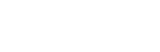
\includegraphics[scale=1]{Figures/Electrodes/fem_illustration.pdf}
\caption{Illustration of the Finite Elements methods for a 1-Dimensional problem (on the left) and a 2-Dimensional problem (on the right). The true solution of the global equations of the system is approximated locally by linear functions on the finite elements. Each linear function is derived from basis functions $\Psi$ associated with each node.}
\label{fig:fem-illustration}
\end{figure}

%All these polynomial functions satisfying the systems of algebraic equations are assembled to form a larger system of equations that models the entire problem. 
%
%over each finite element by a polynomial function. This polynomial function, usually linear, quadratic and cubic, are derived from basis function $\Psi$ associated with each nodes. The approximate numeric solution is expressed:

In the end, the approximate numeric solution $V_h \approx V$ is obtained through numerical linear algebra methods coupled with variational methods minimizing an error function over the whole mesh.

% from stationnary study
%The stationary study consists in solving the stationary electrostatic equations for a considered set of parameters. The solution consists in the values of electric potential $V$ for each vertex of the chosen mesh. This values are interpolated and used to represent the potential on a radial slice of the detector (as seen in figure [fig potential]). It is possible to apply a gradient function to obtain the electric field in the detector (as seen in figure \ref{fig:fid38-enorm}) along with the streamline of the electric field. The streamlines are useful to visualize the direction of the electric field in the crystal and predict the trajectory of the drifting charges in the detector.


\subsection{Mesh Parametrization}
\label{par:mesh-parametrization}

% Dimension space
A cryogenic germanium bolometer equipped with an ionization channel is a 3-Dimensional electrostatics problem. The most straightforward way of building its associated geometry is to reproduce the detector in 3D inside the FEM software. A cylindrical coordinates system centered on an origin $O$ is adapted for this system with the three spatial parameters: $r$ the radius, $\theta$ the angle and $z$ the height. The figure \ref{fig:space-dimension-geometry} displays a cut 3D view of the FID38 design with the cylindrical coordinates system drawn in red. 

\begin{figure}
\centering
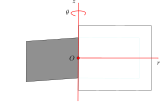
\includegraphics[scale=0.7]{Figures/Electrodes/mesh_3d.pdf}
\caption{Illustration of the 2D-axisymmetric geometry used to simulate the FID38 design. A section of the  The equations are solved on a slice of the detector considering the cylindrical symmetry such that $V(r, \theta, z) = V(r,z)$. The coordinates origin $O(r=0, z=0)$ corresponds to the center of the cylindrical crystal. The mesh is automatically constructed with the "Physics-based" mesh scale of "Fine".}
\label{fig:space-dimension-geometry}
\end{figure}

Although this 3D geometry is valid and yields correct numeric solutions, it is not efficient. Indeed, this 3D geometry does not benefit from the intrinsic cylindrical geometry of the electric potential field $V$ in the resolution $V(r, \theta, z) = V(r,z)$. Instead, the 3D geometry generate a mesh in the entire volume of the detector with a high number of nodes and a lengthy numeric resolution of the electrostatics equations.

% 2D axysymmetry
An alternative approach is consider a resolution on a radial slice of the detector with built-in cylindrical symmetry. Inside the FEM software, the geometry is built with the 2D-axisymmetry. The figure \ref{fig:space-dimension-geometry} displays this radial section. The equations are now solved over a 2D mesh also yielding the correct numeric solution. A major advantages of the 2D-axisymmetry over the 3D geometry is the much lower number of vertices composing the mesh. This translates into significantly shorter resolution times. The amount of scanning studies presented in the next chapter \ref{ChapterElectrodesScan} is a direct results of this gain in time. The main drawback to the use of the 2D-axisymmetry is by definition the need to have a system respecting the cylindrical symmetry. In this work, several characteristics of the detector were ignored in the electrostatics simulation due to not respecting the symmetry: the Teflon clamps holding the crystal, the NTD thermal sensor and the aluminium wire-bridges between the aluminium deposits. There influence on the whole system is considered negligible. In order to study the local effects of these non-symmetric features, the 3D geometry should be used.


% Mesh Parametrization
When solving a problem with the finite element method, the choice of the meshing is essential. Due to the FEM approximating the analytical solution with a numerical approach over the vertices of the mesh, the meshing should be well constructed to assure a precise estimation. For a given physic system, the analytical solution can be more precisely approximated as the number of vertices is increased. However, a high number of vertices induces an equal number of local numerical solving. The COMSOL software offers an automatic optimization of the meshing which adapts the size of meshing to the geometry of the system. Such an optimized mesh is presented on the figure \ref{fig:space-dimension-geometry}. There are a lot of vertices near small geometric features such as in vicinity of the aluminium rings of the electrodes at the surface of the Ge crystal. This assures that a rapidly varying electric field is correctly mapped. At the same time, there are only few vertices at location where the electric field is almost uniform as in the bulk of the crystal.

% Automatic Meshing
This optimization of the meshing is possible with the “Physics-based” option of COMSOL which automatize the meshing process taking as single parameter the mesh scale. Simulation of the reference designs PL38 and FID38 were ran with different mesh scales and the results are presented in table \ref{tab:mesh-scale}. There are nine mesh scales proposed by COMSOL, starting from the "Extremely Coarse" scale with a low number of simplex, a low accuracy and very quick run time, and continuing with increasingly refined scale to the "Normal" scale, which should result in a trade-off between simulation time and precision, eventually reaching the "Extremely Fine" scale with a very high precision obtained after a long calculation time. 

\begin{table}[]
\centering
\resizebox{\textwidth}{!}{%
\begin{tabular}{c|rrr|rrr}
\multirow{2}{*}{Mesh Scale} & \multicolumn{3}{c|}{Planar38} & \multicolumn{3}{c}{FID38} \\ \cline{2-7} 
 &
  \multicolumn{1}{c}{\# Triangles} &
  \multicolumn{1}{c}{Capacitance {[}pF{]}} &
  \multicolumn{1}{c|}{Relative Error {[}\%{]}} &
  \multicolumn{1}{c}{\# Triangles} &
  \multicolumn{1}{c}{Capacitance {[}pF{]}} &
  \multicolumn{1}{c}{Relative Error {[}\%{]}} \\ \hline \hline
Extremely Fine              & 37837    & 14.923   & 0      & 106028   & 19.217  & 0     \\
Extra Fine                  & 11721    & 14.923   & 0      & 41991    & 19.223  & 0.03  \\
Finer                       & 6306     & 14.923   & 0      & 29996    & 19.222  & 0.02  \\
Fine                        & 4368     & 14.923   & 0      & 22504    & 19.232  & 0.08  \\
Normal                      & 4258     & 14.923   & 0      & 22340    & 19.232  & 0.08  \\
Coarse                      & 2472     & 14.924   & 0.01   & 15288    & 19.263  & 0.24  \\
Coarser                     & 1303     & 14.934   & 0.07   & 7596     & 19.475  & 1.34  \\
Extra Coarse                & 1260     & 14.964   & 0.27   & 7915     & 19.693  & 2.47  \\
Extremely Coarse            & 1937     & 15.037   & 0.76   & 19714    & 19.625  & 2.12 
\end{tabular}%
}
\caption{Scanning the mesh scale of the simulated PL38 and FID38 design. The control values are the number of triangles forming mesh, the first diagonal term of the Maxwell capacitance matrix and the relative error on the capacitance calculation with the "Extremely Fine" scale chosen as reference.}
\label{tab:mesh-scale}
\end{table}

As expected, the more refined the scale is and the more triangles are used for the simulation (except for Extremely Coarse, maybe a non-optimized meshing algorithm is in use). As the FID38 design has more electrodes of small size than the simpler PL38 design, the mesh is generated with more simplex. It is consistent with the fact that the simulation of the PL38 design run quicker than for the FID38.
In order to estimate the accuracy of the simulation scanning over the different scales, a capacitance value corresponding to the first diagonal term of the Maxwell capacitance matrix (see the later paragraph \ref{par:capacitance-matrix}) is evaluated as control quantity. Additionally, a percentage of the relative error on the capacitance calculation is given. The capacitance of the "Extremely Fine" scale is chosen to be the reference for this relative error. By definition, the relative error of the "Extremely Fine" is zero. Table \ref{tab:mesh-scale} shows that as the scale is more refined, the capacitance is getting closer to the reference capacitance.
In the case of the PL38, the relative error starts at \SI{0.78}{\percent} and eventually reaches zero for the "Normal" scale. Concerning the FID38 design, the relative error is greater for all scales compared to the PL38. This may be due to the more complex geometry. Although the error is superior to \SI{1}{\percent} for the less refined scales, from the "Normal" scales the error is inferior to \SI{0.1}{\percent}.
Considering that the "Normal" and "Fine" possesses a similar number of simplex and resolution time, the simulation presented in this work are ran with the "Fine" scale. The capacitance calculation are affected by a relative error of about \SI{0.1}{\percent}. 


\subsection{Geometry and Physics of the PL38 and FID38 Simulation}
%\subsection{Modelization of a RED detector}

% Intro
%This work aims at discovering and quantifying the impact of the design of the electrodes upon the ionization channel performance. Multiple geometries were simulated with common parameters and sometimes their own specific parameters. In this work, two reference electrode geometries are simulated: the "PL38" and “FID38” designs.
This paragraph is dedicated to building the geometry and defining the electrodes of the PL38 and FID38 design simulations. The description of these detector designs is illustrated with the annotated schemes \ref{fig:pl38-scheme} for the PL38 and \ref{fig:fid38-scheme} for the FID38. These scheme are used as reference for building the geometry in the FEM software. The schemes are not entirely at scale and are thus accompanied with the lists of the parameter values \ref{tab:pl38-default-parameters} and \ref{tab:fid38-default-parameters} for the PL38 and FID38 designs respectively.

\begin{figure}
\centering
\includegraphics[scale=1]{Figures/Electrodes/scheme_pl38.pdf}
\caption{
Cross-section scheme of the PL38 detector design. The scheme is not at scale and the dimensions and parameters of this design are listed in the table \ref{tab:pl38-default-parameters}. The copper chassis is represented by the electrically grounded rectangle. It is separated from the germanium crystal by the vacuum colored light-blue. The two aluminium electrodes are represented in black at the surface of the crystal. The default polarization of PL38 is $(V_A, V_B) = (+1, -1) \ \si{\volt}$. The colored volumes inside the crystal are drawn from electric field lines with common start and end points.
}
\label{fig:pl38-scheme}
\end{figure}

\begin{table}[]
\centering
%\resizebox{\textwidth}{!}{%
\begin{tabular}{l c S}
Parameter                                   & Symbol        & {Default Value} \\ \hline \hline
Ge crystal Height                           & $H_{Ge}$      & \SI{10}{\mm}  \\
Ge crystal Radius                           & $R_{Ge}$      & \SI{15}{\mm}    \\
Distance between crystal and copper chassis & $d_{Cu}$      & \SI{3}{\mm}     \\
Electrode Thickness                         & $h_{Al}$      & \SI{1}{\micro\meter}   \\
Radius of the central NTD hole    & $r_{center}$   & \SI{1.5}{\mm}   \\
Corner length & $L_{lat}$ & \SI{2}{\mm}  \\
Main Voltage Bias                           & $V_{bias}$    & \SI{2}{\volt}      \\
Symmetric factor of the voltage bias        & $S_{bias}$    & {$0.5$}         
\end{tabular}
%}%
\caption{List and Value of the default parameters for the PL38 design.}
\label{tab:pl38-default-parameters}
\end{table}

\begin{figure}
\centering
\includegraphics[scale=1]{Figures/Electrodes/scheme_fid38.pdf}
\caption{
Cross-section scheme of the FID38 detector design. The scheme is not at scale and the dimensions and parameters of this design are listed in the table \ref{tab:fid38-default-parameters}. The copper chassis is represented by the electrically grounded rectangle. It is separated from the germanium crystal by the vacuum colored light-blue. The aluminium pads and rings are represented in black at the surface of the crystal and labeled according to their electrode of attribution. The default polarization of FID38 is $(V_A, V_B, V_C, V_D) = (-0.25, +1, +0.25,  -1) \ \si{\volt}$. The colored volumes inside the crystal are drawn from electric field lines with common start and end points.
}
\label{fig:fid38-scheme}
\end{figure}

\begin{table}[]
\centering
%\resizebox{\textwidth}{!}{%
\begin{tabular}{l c S}
Parameter                                   & Symbol        & {Default Value} \\ \hline \hline
Ge crystal Height                           & $H_{Ge}$      & \SI{10}{\mm}  \\
Ge crystal Radius                           & $R_{Ge}$      & \SI{15}{\mm}    \\
Distance between crystal and copper chassis & $d_{Cu}$      & \SI{3}{\mm}     \\
Electrode Thickness                         & $h_{Al}$      & \SI{1}{\micro\meter}   \\
Electrode Width                             & $w_{Al}$      & \SI{80}{\micro\meter}  \\
Radius of the innermost planar electrode    & $r_{center}$   & \SI{0.25}{\mm}   \\
Width of bare Ge crystal on corners      & $w_{bare}$    & \SI{0.3}{\mm}  \\
Width of the outermost veto electrode    & $w_{outer}$    & \SI{0.08}{\mm}  \\
Number of planar electrodes                 & $n_{plan}$  & {$7$}             \\
Number of lateral electrodes                & $n_{lat}$ & {$2$}             \\
Interdistance of Planar electrodes          & $d_{plan}$  & \SI{1.98}{\mm}  \\
Interdistance of Lateral electrodes         & $d_{lat}$ & \SI{2.40}{\mm}  \\
Equatorial distance & $d_{eq}$ & \SI{2}{\mm}  \\
Main Voltage Bias                           & $V_{bias}$    & \SI{2}{\volt}      \\
Ratio Veto/Main voltage bias                & $R_{veto}$    & {$-0.25$}         \\
Symmetric factor of the voltage bias        & $S_{bias}$    & {$0.5$}         
\end{tabular}
%}%
\caption{List and Value of the default parameters for the FID38 design.}
\label{tab:fid38-default-parameters}
\end{table}

% Common geometry
The two PL38 and FID38 detector designs use cylindrical germanium crystals of height $H_{Ge} = \SI{10}{\mm}$ and radius $R_{Ge} = \SI{15}{\mm}$ as absorber. The mass of these crystals are about \SI{38}{\g} hence the name of the the designs as to differentiate them from more massive \SI{200}{\g} and \SI{800}{\g} EDELWEISS detectors. Each crystal is surrounded by an hollow cylindrical chassis which is electrically grounded to \SI{0}{\volt}. This copper chassis is spaced from the crystal by a distance $d_{Cu} = \SI{3}{\mm}$ of vacuum.
% Permittivty
The vacuum is simulated with a relative electric permittivity of $\epsilon_r(\textsf{Vacuum}) = 1$ and the germanium crystal possesses a much higher value of $\epsilon_r (\textsf{Ge}) = 16.3$. Although present in real detectors to maintain the crystal, Teflon clamps are not simulated. Indeed, their influences is considered negligible due to their small size and low permittivity $\epsilon_r(\textsf{Teflon})=2.1$.
% NTD location
Similarly, the real detectors inspired by the PL38 and FID38 design should possess NTD thermal sensors but these thermistances are not simulated. Their predicted gluing locations are annotated on the scheme. These location are chosen as to reduce the contact of the NTD with the aluminium electrode. For the PL38 design, the NTD is located in the central hole of the top electrode in contact with the bare germanium surface. For the FID38 design, the NTD should be glued on top of a veto electrode ring. As such, a majority of the NTD surface should be in contact with the bare germanium surface while perturbing the electric field very locally in the top veto volume.
% Difference PL38 FID38
The main difference between the two detector design concern the number and shape of aluminium electrodes. The PL38 design holds its name from the two full planar electrodes while the FID38 design features four fully inter-digitized electrodes. The simpler PL38 design is presented first followed by the description of the more complex FID38 design.

%The electrodes are simulated by extruded annuli, resembling thin rings, composed of aluminium of height $h_{Al}=0.01[mm]$ and width $w_{Al}=0.08mm$. Real electrodes possess a much lower height of about 50nm. However, this value is so low that the meshing is invariably messed up.

%PL38
The ionization channel of the PL38 detector design consists in two collecting electrodes readily visible of the scheme \ref{fig:pl38-scheme}. Each electrode is denominated by their location on the top or bottom surface but for more clarification we can define the following convention for the electrode denomination and indexes in this work:
\begin{equation}
\label{eq:pl38-convention}
\lbrace \textsf{Top}, \textsf{Bottom} \rbrace
\Leftrightarrow 
\lbrace A, B \rbrace
\Leftrightarrow
\lbrace 1, 2 \rbrace
\end{equation}
Each electrode is basically a continuous aluminium deposit on the full surface with some extension on the lateral surface. The extension length on the lateral surface is noted $L_{lat}$ with a default value of \SI{2}{\mm}. While the bottom electrode $B$ covers the full bottom surface of the crystal, the top electrode $A$ features a central hole. This hole is meant to provide the NTD thermal sensor with a bare germanium as to increases the fraction of athermal phonon as discusses in the dedicated paragraph \ref{par:athermal-phonons}. The hole is circular of radius $r_{center}$. Its default value of \SI{1.5}{\mm} is meant to host a NTD of small standard area \SI{2 x 2}{\mm}.

% FID38
The design FID38 has a more complex ionization channel composed of four electrodes labeled $A$ through $D$. The denomination of these electrodes in this work follows the convention:
\begin{equation}
\label{eq:fid38-convention}
\lbrace \textsf{Top Veto}, \textsf{Top Collect}, \textsf{Bottom Veto}, \textsf{Bottom Collect} \rbrace
\Leftrightarrow 
\lbrace A, B, C, D \rbrace
\Leftrightarrow
\lbrace 1, 2, 3, 4 \rbrace
\end{equation}
 As displayed on the scheme \ref{fig:fid38-scheme}, each electrode is an association of aluminium pads and rings. 
% Association
For real detectors, this association is made by linking the aluminum deposits with aluminium wires bridging over the germanium surface as discussed in the paragraph \ref{par:wire-bounding}.
Inside the electrostatic simulation software, multiple deposits can be assigned to the same electric terminal thus sharing their potential and charges. It is therefore possible to avoid the simulation of the wire-bonding bridges between the different aluminium deposits.
% Deposit geometry
These deposits consists in two pads and multiples rings whose shape depends on several parameters. The radius of the circular central pads on the top and bottom surface is noted $r_{center}$ and is by default set to \SI{0.25}{\mm}. The width of the concentric aluminium rings is by default set to the minimal value of $w_{Al} = \SI{80}{\micro\meter}$. The outermost planar rings are attributed a specific independent width $w_{outer}$ with the same default value. The number of total separated deposits, pads and rings, is noted $n_{plan}$ for the planar surface and $n_{lat}$ for the lateral surfaces. The default configuration sets these numbers to $n_{plan}=7$ and $n_{lat}=2$. The radius of the outermost ring is limited to the radius of the germanium crystal minus a band of width $r_{edge}=\SI{0.3}{\mm}$. This comes from the limits of the aluminium deposition technique employed: it is not possible to have a thin aluminium electrode at less than \SI{0.3}{\mm} from the edge of the planar surface of the germanium crystal. The concentric aluminium rings are spaced evenly on the planar surfaces with a distance $d_{plan}=\SI{2.40}{\mm}$ between their center. On the lateral surface, aluminium rings respect the mirror symmetry with the equator of the cylindrical germanium crystal. The two most centered lateral electrodes, deemed equatorial rings, are distant from each other by $d_{eq}=\SI{2}{\mm}$. The remaining lateral electrodes are evenly separated by the lateral spacing of default value $d_{lat}^{lateral}=\SI{1.98}{\mm}$ between the equatorial rings and the crystals corners.
% Deposit attribution to electrodes
Now that the aluminium deposits are defined, they can be attributed to an electrode. The electrodes respect a top-bottom symmetry with $A$ and $B$ being the top electrode with $C$ and $D$ being their bottom counterpart. The electrodes $B$ and $D$ corresponds to the main collecting electrodes, also called collect electrodes. Their function is to record the signal induced by recoils located in the bulk of the crystal. The electrodes $A$ and $C$ corresponds to auxiliary veto electrodes, also called veto electrodes. Their function is to collect the electric charges produces near the surface of the absorber. This surface tagging ability is the motivation behind the FID-like detector designs and is discussed in the paragraph \ref{par:surface-tagging}. In order to create a usable veto volume on the surface, the equatorial rings, the outermost planar electrodes and the central pads are attributed to the veto electrodes $A$ and $C$. The remaining rings are attributing in order to obtain a succession of collect and veto electrodes. This attribution process imposed constraints on the number of planar and lateral aluminium deposits. Indeed, the interleaving of collect and veto deposits necessitates $n_{plan}$ to be an odd integer and $n_{lat}$ to be even.

% Polarization
For the PL38 and FID38 designs, the polarization of the electrodes is controlled by several parameters. First is the voltage bias of the detector, noted $V_{bias}$, corresponding to the voltage between the two main collecting electrodes. For both design, its default value is \SI{2}{\volt}. Then comes the bias symmetry factor $S_{bias}$ representing the symmetry of the top and bottom electrodes potential in respect to the \SI{0}{\volt} ground voltage. At the default value of $0.5$, polarization are considered symmetric with opposite-side electrodes having opposite electric potential.
With this two parameters, the polarization of the PL38 design is expressed as:
\begin{equation}
\label{eq:fid-polarization}
\begin{cases}
\displaystyle
V_A = V_{bias} \cdot S_{bias}
\\
\displaystyle
V_B = - V_{bias} \cdot (1 - S_{bias})
\end{cases}
\Rightarrow
\textsf{with } S_{bias} = 0.5,
\begin{cases}
\displaystyle
V_A = V_{bias} / 2
\\
\displaystyle
V_B = - V_{bias} / 2 
\end{cases}
\end{equation}
The default polarization of the PL38 design corresponds to:
\begin{equation}
\left( V_A, V_B \right) = (+1, -1) \ \si{\volt}
\end{equation}
As such, the top electrode $A$ should collect the electrons of negative electric charge while the bottom electrode $B$ collects the positively charged holes.

% Naive calculation of the electric field inside the crystal ?

% Polarization
With two auxiliary veto electrodes, the FID38 necessitate an additional parameters to fix the polarization of its electrodes. The veto ratio factor noted $R_{veto}$ is used to define the voltage difference between the main collecting and the auxiliary veto electrodes. Its default value for the FID 38 design is $-0.25$. The polarization of the FID38 design is therefore expressed as:
\begin{equation}
\label{eq:fid-polarization}
\begin{cases}
\displaystyle 
V_A = V_{bias} \cdot \left( S_{bias} - \frac{\left( 1 + R_{veto}\right)}{2}\right)
\\
\displaystyle
V_B = V_{bias} \cdot S_{bias}
\\
\displaystyle
V_C = V_{bias} \cdot \left( S_{bias} + \frac{\left( -1 + R_{veto}\right)}{2}\right)
\\
\displaystyle
V_D = - V_{bias} \cdot (1 - S_{bias})
\end{cases}
\Rightarrow
\textsf{with } S_{bias} = 0.5,
\begin{cases}
\displaystyle 
V_A = - R_{veto} \cdot V_{bias} /2
\\
\displaystyle
V_B = V_{bias} /2 
\\
\displaystyle
V_C = R_{veto} \cdot V_{bias} /2
\\
\displaystyle
V_D = -  V_{bias}/2
\end{cases}
\end{equation}
The default polarization of the FID38 design corresponds to:
\begin{equation}
\label{eq:fid38-polarization-default}
\left( V_A, V_B, V_C, V_D \right) = (-0.25, +1, +0.25, -1) \ \si{\volt}
\end{equation}

% Naive calculation of the electric field inside the crystal ?

% Note on simulation
The electric equations are solved only in the insulators domains corresponding to the germanium crystal and the surrounding vacuum inside the copper chassis. The aluminium electrodes are set to a fixed potential and thus their interior is excluded from the simulation. 


\subsection{Weighted Potential Study}
\label{par:weighting-potential}

The following discussion is the continuation of the paragraph \ref{par:shockley-ramo} introducing the signal generation on the electrodes by drifting electric charges with the Shockley-Ramo theorem. It concluded with the equation \ref{eq:ramo-induced-charge} modeling the signal generated on the electrodes of the detector. This signal induced on the electrode $X$ depends on its weighting potential $\Phi_X$ at final positions of the drifting carriers in the crystal $\vec{r}_{q, f}$. This paragraph presents the study of the weighting potentials associated with the ionization channel of the PL38 and FID38 design (in their default configurations). Electrodes are denominated by the labels $X,Y \in \{ A, B \}$ for the PL38 design or $X,Y \in \{ A, B, C, D \}$ for the FID38 design.

For each successive electrode $X$, all the electrodes are grounded except for the electrode $X$ which is fixed at the unitary potential:
\begin{equation}
\begin{cases}
V_X = \SI{1}{\volt} \\
\forall Y \neq X, V_Y = \SI{0}{\volt}
\end{cases}
\end{equation}
The electric potential fields $V$, solutions to the resulting electrostatics equations, corresponds to the weighting potentials $\Phi_X$. The total weighting potential $\Phi_T$ is calculated with the equation \ref{eq:twp}.
 
The figure \ref{fig:pl38-fid38-weighting-potential} displays several graphics illustrating the weighting potentials of the PL38 design (in the left column) and the FID38 design (in the right column).
In the first row, the graphics are the color maps of $\Phi_A$ for the PL38 and $\Phi_B$ for the FID38 design. The pattern drawn by the potentials are consistent with the geometry of the electrodes. 
 In the second row, the color maps of the total weighting potential $\Phi_T$ are plotted for both designs. The last row are graph presenting weighting potentials $\Phi_X$ as function of the height $z$ on a single linear trajectory at a radius $r=\SI{12.65}{\mm}$ in the germanium crystal.

% A map of the weighted potential associated to each electrode is obtained by fixing the potential of the considered electrode to the unitary value of 1V and grounding all the other terminals. (see left of  figure [Weighted potential]). The total weighted potential is obtained by summing over the different electrodes. (see left of  figure [Weighted potential]).

\begin{figure}
\begin{minipage}{0.48\textwidth}
\centering
\includegraphics[scale=0.5]{Figures/Electrodes/pl38_swp.png}
\includegraphics[scale=0.5]{Figures/Electrodes/pl38_twp.png}
\includegraphics[scale=0.5]{Figures/Electrodes/pl38_wp_plot.png}
\end{minipage}
\hfill\vline\hfill
\begin{minipage}{0.48\textwidth}
\centering
\includegraphics[scale=0.5]{Figures/Electrodes/fid38_swp.png}
\includegraphics[scale=0.5]{Figures/Electrodes/fid38_twp.png}
\includegraphics[scale=0.5]{Figures/Electrodes/fid38_wp_plot.png}
\end{minipage}
\caption{Graphics related to the weighting potentials for the default configuration of the PL38 design (in the left column) and the FID38 design (in the right column). The graphics in the first row represents the weighting potential associated with the top electrode $A$ of PL38 design and the top collect electrode $B$ of the FID38 design. The graphics of the second row are color maps of the total weighting potential of the two designs. Grey contours are plotted to appreciate small variation in the bulk of the crystal. On the last row are plotted the weighting potential $\Phi_X$ as functions of the $z$-coordinates on vertical lines between the main collecting electrodes on the radius $r=\SI{12.65}{\mm}$ . These vertical lines are plotted in the previous color maps in black for the PL38 design and red for the FID38 design.}
\label{fig:pl38-fid38-weighting-potential}
\end{figure}

The graphics of the first and third row show that the weighting potentials $\Phi_X$ are equals to one on their associated electrode $X$ and are null on all others electrodes $Y$. These observations verify the generalization of the properties of the weighting potential of a single particle of equation \ref{eq:ramo-particle} to a polarized electrode $X$ of any shape. We can admit that for any electrode $X$ their weighting potential $\Phi_X$ has the following properties:
\begin{equation}
\label{eq:ramo-electrode}
\begin{cases}
\Phi_X \left( \vec{r} \in \Sigma(X) \right) = 1 \\
\forall Y \neq X: \Phi_X \left( \vec{r} \in \Sigma(Y) \right) = 0
\end{cases}
\end{equation} 
where $\Sigma(X)$ is the surface of the the electrode $X$.

%While the red color indicate a total weighted potential $\phi_T$ which tends to 1, the color blue is associated to an inferior total weighted potential.

The total weighting potential $\Phi_T$ of the PL38 design is almost uniform in the bulk of the crystal with an average value of $\langle \Phi_T \rangle = 0.98$ close to 1. As such, this detector acts as a very good Faraday cage. In the crystal, $\Phi_T$ is maximal near the electrodes and minimal with $\Phi_T = 0.94$ at the equator. This comes from the influence of the grounded chassis. Indeed, near the equator, a fraction ($1-0.94=0.06$) of the signal is induced on the chassis. The very high total potential can be explained by the full planar electrodes of the PL38 design shielding the interior of the crystal from the copper chassis. As as result, in the worst case scenario with charge carriers trapped near the equator, only \SI{6}{\percent} of the induced charge is lost.

For the FID38 design, the total weighting potential is globally lower with an average value of $\langle \Phi_T \rangle = 0.95$. Similarly, it tends to 1 near the electrodes and fall in regions with higher influence of the copper chassis. These regions seems to be the bare germanium surfaces between the aluminium rings an in particular the corners of the crystal. The function of Faraday cage of the FID38 is still considered as excellent even if less than the PL38 design.

% while it is increasing near the electrodes. According to the Shockley-Ramo theorem, electron-holes pairs created very near an electrode are inducing a signal almost entirely in the A,B,C,D electrode. However, for pairs created in the bulk of the crystal, a fraction  of the signal is induced in the copper chassis outside of the crystal. As a result, the detector is not a perfect Faraday Cage, but is approaching its properties as the minimum total weighted potential in the crystal is 0.94.  

%{ color{blue} Discussion on the loss of energy in the case of trapping as a result of a total weighted potential inferior to 1. Rough estimation of the limit on the intrinsic resolution of the ionization resolution for several fraction of trapping per recoil.}

% Following the shockley ramo paragraph
%We can now follow the discussion on the Shockley-Ramo theorem with illustration. 

% Induced signal on the electrodes
With the calculation of the weighting potential $\Phi_X$, it is now possible to predict the induced current signal from the final position of the charge carriers thanks to equation \ref{eq:ramo-induced-charge}. These finals drift positions of the electrons and holes are estimated in the next paragraph \ref{par:stationnary-study}.

%In the case of the Planar38, the charges are collected by the top and bottom electrodes. We can introduce the electric charge vector associated to the Planar38:

For now, we introduce the vector formalism used to model the ionization signal generation. All the induced electric charge $Q_X$ and the electric potential $V_X$ of the electrodes of a detector are gathered in two vectors: the induced charge vector $\vec{Q}$ and the voltage signal vector $\vec{V}$. With two electrode $A$ and $B$, these vectors are expressed for the PL38 design as:
\begin{equation}
\vec{Q}^{PL38} =
\begin{bmatrix}
Q_{A} \\ Q_{B}
\end{bmatrix}
\quad
\textsf{and}
\quad
\vec{V}^{PL38} =
\begin{bmatrix}
V_{A} \\ V_{B}
\end{bmatrix}
\end{equation}
The FID38 possesses two main collecting electrodes $B, D$ and two veto electrodes $A, C$. The charge and voltage vectors become:
\begin{equation}
\vec{Q}^{FID38} =
\begin{bmatrix}
Q_{A} \\ Q_{B} \\ Q_{C} \\ Q_{D}
\end{bmatrix}
\quad
\textsf{and}
\quad
\vec{V}^{FID38} =
\begin{bmatrix}
V_{A} \\ V_{B} \\ V_{C} \\ V_{D}
\end{bmatrix}
\end{equation}


\subsection{Stationnary Study}
\label{par:stationnary-study}
\label{par:fiducial-volume}

The stationary study consists in solving the stationary electrostatic equations for a considered set of parameters. In this chapter, the PL38 and FID38 designs are simulated with the default parameters listed in the table \ref{tab:pl38-default-parameters} and \ref{tab:fid38-default-parameters} respectively. The figure \ref{fig:pl38-fid38-steady-state} plots several quantities derived from these resolution.

\begin{figure}
\begin{minipage}{0.49\textwidth}
\centering
\includegraphics[scale=0.5]{Figures/Electrodes/pl38_potential.png}
\includegraphics[scale=0.5]{Figures/Electrodes/pl38_enorm.png}
\includegraphics[scale=0.5]{Figures/Electrodes/pl38_enorm_hist.pdf}
\end{minipage}
\hfill\vline\hfill
\begin{minipage}{0.49\textwidth}
\centering
\includegraphics[scale=0.5]{Figures/Electrodes/fid38_potential.png}
\includegraphics[scale=0.5]{Figures/Electrodes/fid38_enorm.png}
\includegraphics[scale=0.5]{Figures/Electrodes/fid38_enorm_hist.pdf}
\end{minipage}
\caption{
Graphics summarizing the resolution of the electrostatic equations for the  simulated PL38 (on the left) and FID38 designs (on the right) in their default configuration. The graphics of the first row are colored contours of the electric potential $V$. The graphics of the second row are the color maps of the norm of the  electric field $|| \bm{E} ||$  with superimposed black electric field lines. On the last row are the density histograms and cumulative distribution functions of $|| \bm{E} ||$ over the crystal volume.
}
\label{fig:pl38-fid38-steady-state}
\end{figure}

% Explanation Electric potential
For each design, the simulation yields an electric potential field $V(r,z)$ on the radial slice of the detector. These electric potential are represented with a color map with the first row of graphics in figure \ref{fig:pl38-fid38-steady-state}. 
% Explanation Electric field and field lines
By applying a gradient function, the electric field $\bm{E}(r,z)$ is calculated in the detector. The second rows of graphics are color maps of the magnitude $||\bm{E}(r,z)||$ of the electric field. Superimposed in black are the electric field lines associated (discussed thoroughly later in this paragraph).
% Explanation histogram and cdf
The graphics of the last row of the figure \ref{fig:pl38-fid38-steady-state} corresponds to the density histogram of the electric field norm $||\bm{E}(r,z)||$ over the whole crystal volume. The histograms are completed with the cumulative distribution function. The histograms and cumulative are computed with the weighting function:
\begin{equation}
\label{eq:rotation-weight}
W(r,z) = 2\pi \times r
\end{equation}
This is a consequence of the use of the 2D-axisymmetry: estimating a volume from an area of the radial slice necessitate to revolve it by $2\pi$. Similarly, the later estimation of the fiducial volume is based on this weighting function.

% PL38 observation
The design PL38 displays equally spaced equipotential lines in the crystal volume with some slight deformation on the lateral surface due to shape of the electrodes. As a result, the electric field norm is uniform on almost the whole crystal volume. Electric field lines are vertical in the bulk of the crystal with some curve on the periphery. There are some regions of low magnitude in the corners of the crystal and under the central hole of the top electrode $A$. The field lines are diverging from these low magnitude regions to join the electrodes or the grounded chassis. The density histogram of $||\bm{E}||$ is consistent with these observations: the distribution peaks at \SI{2}{\volt\per\cm} with slight broadening of the distribution at higher or lower values. The value of the peak equals the naive calculation of the electric field $E_{naive}$ between two infinite plate of potential $V_A=\SI{+1}{\volt}$ and $V_B=\SI{-1}{\volt}$ spaced by a distance $H_{Ge}=\SI{10}{\mm}$:
\begin{equation}
\label{eq:pl38-naive-efield}
|| \bm{E}_{naive}^{PL38} || = \left| \frac{V_A - V_B}{H_{Ge}} \right| = \SI{2}{\volt\per\cm}
\end{equation}
The higher tail of the distribution with $||\bm{E}||> \SI{2}{\volt\per\cm}$ corresponds to the peripheral volume of the crystal, on the lateral surface. Indeed, the distance between the electrodes is smaller on the lateral side due to the electrode extension of length $L_{lat} = \SI{2}{\mm}$ resulting into a higher electric field norm. The lower tail is explained by the presence of the low magnitude central and corner regions.

% FID38
For the FID38 design, the electric potential field $V(r,z)$ is rapidly changing in the vicinity of the aluminium deposits near the surface. The equipotential lines shows the alternation of the polarization of the electrodes on the surface of the crystal. This FID polarization shape the electric field near the surface of the crystal. Indeed, surface field lines join same-sided collect and veto electrodes. Due to the electric peak effect created by the aluminium deposit, the magnitude of the electric field is high near the surface. In the bulk of the crystal, the magnitude is of lower value with a uniform electric field demonstrated by the vertical field lines. Interestingly, the electric field is null between $1$ to \SI{2}{\mm} deep into the crystal under the aluminium deposits attributed to the veto electrodes $A$ and $C$. The electric field lines diverges from these low magnitude regions.
The volumetric density distribution of the norm of the electric field $||\bm{E}||$ associated to the FID38 design is broader than the distribution of the PL38 design. Indeed, for the FID38, \SI{15}{\percent} of the volume has a magnitude superior to \SI{2}{\volt\per\cm}. This higher tail of the distribution is explained by the high intensity of the electric field near the surface due to the electric peak effects. As this tail has no clear features and asymptotically reach a density of zero it is not represented on the graphics. Indeed, the presented density histogram focuses on lower magnitude which features multiples peaks between $0.5$ and \SI{1}{\volt\per\cm}. These values corresponds to the bulk volume of the detector without the low magnitude regions. The regions of low electric field norm are associated with the lower tail of the distribution.
%The majority of the crystal seems to be subject to a electric field of norm $\approx 200 V/cm$. Each peak can be link to specific region in the crystal with equal norm. The low-norm regions appears to be negligible in proportion.

As reference for the magnitude of the electric field, we can naively compute the expected $||\bm{E}||$ in the FID38 crystal similarly to the PL38 design in equation \ref{eq:pl38-naive-efield}. Far from the surface, the two top (resp. bottom) interleaved electrodes $A$ and $B$ (resp. $c$ and $D$) would be perceived as a planar electrode of electric potential $V_{top} = (V_B + V_A)/2 = \SI{0.375}{\volt}$ (resp. $V_{bottom} = (V_D + V_C)/2 = -\SI{0.375}{\volt}$). Assuming the center of the crystal at $z=0$ being sufficiently far from the surface, the norm of the electric field would be:
\begin{equation}
\label{eq:fid38-naive-efield}
|| \bm{E}_{naive}^{FID38} || = \left| \frac{V_{top} - V_{bottom}}{H_{Ge}} \right| = \SI{0.75}{\volt\per\cm}
\end{equation}
This value corresponds to one of the peak of the magnitude distribution which can therefore be attributed to the central bulk of the crystal.

%% Enorm
%FROM THE SCAN CHAPTER \\
%The magnitude of the electric field in the bulk of the crystal decreases with the rising $R_{veto}$. Far from the electrodes, the interleaved same-sided veto and collect electrode rings appears to have the influence of an equivalent planar electrode of electric potential $V=\frac{V_B + V_A}{2}$ and so the perceived electric field norm in the bulk is $E = \frac{V_B + V_A - V_D - V_C}{2 H_{Ge}}=...$ (this calculation should appears when introducing the norm of the electric field and discussing the figure at default value. The calculation explain the phenomenon observed now during the scan over $R_{veto}$).
%{\color{red} [Comparison to enorm threshold, to do later.]}

% Electric field lines
The electric field lines in the PL38 and FID38 deign are drawn in black on the graphics of the second row of figure \ref{fig:pl38-fid38-steady-state}. By construction, the field lines are parallel to the direction of the electric field $\bm{E}(r,z)$ and perpendicular to the equipotential of the $V(r,z)$ field. 
%The electric field is colinear with the Lorentz force $\bm{F}$ applied on an electric charge $q$ drifting in the crystal:
%\begin{equation}
%\bm{F} = q \cdot \bm{E} + q \cdot ( \bm{v} \wedge \bm{B}) = q \cdot \bm{E}
%\end{equation}
%with $\bm{v}$ the velocity of the charge, and $\bm{B}=\SI{0}{\tesla}$ the magnetic field considered null for the operation of the detectors. As a result, the electric field lines corresponds to the trajectories of the drifting charges in the crystal with two major assumption: the Lorentz force is the sole force applied on the particles and the inertia of the particles is negligible. As discussed in the previous paragraph \ref{par:charge-drift}, these assumptions are incorrect. However, the electric field lines still provide an good approximation of the trajectories. This approximation is very close for the holes drift and less reliable for the electrons drift due to their transversal movement discussed in the paragraph \ref{par:charge-drift}.
As explained in the paragraph \ref{par:charge-drifting}, the motion of the holes follows the electric field lines while the electrons propagates in oblique directions in respect to the vertical axis. For the sake of clarity, assuming that the field lines are the trajectories of all the drifting charge carriers is denominated as the "assumption of ideal charge drift".
% Link to Shockley Ramo theorem
This ideal drift is used to model the ionization signals in a detector. The electric charge $Q_X$ induced on an electrode $X$ of the detector is calculated from its associated weighting potential field $\phi_X(\vec{r})$ according to the equation \ref{eq:ramo-induced-charge}. This application of the Shokley-Ramo theorem discussed in the paragraph \ref{par:shockley-ramo} is based on the knowledge of the final positions of the electric charges $\vec{r}_{e^-,f}$ and $\vec{r}_{h^+,f}$. The assumption of ideal drift indicates that these final positions corresponds to the start and end points of the electric field line passing by the position of the ionizing recoil $\vec{r}$.

The extremities of the electric fields in the germanium crystal are bound to be either a bare germanium surface or an electrode. While the weighting potential $\Phi_X$ associated with an electrode $X$ is variable on the whole bare surface of the germanium, its value are fixed to either 0 or 1 on the surface of the electrodes according to the properties \ref{eq:ramo-electrode} of $\Phi_X$. 
We can therefore classify the electric field lines according to their start and end points and their associated weighting potential $\Phi_X$ for each of the electrode $X$. For each class of field lines, a part of the crystal volume is drawn in the cross-section schemes \ref{fig:pl38-scheme} and \ref{fig:fid38-scheme}. Recoils yielding a fixed ionization energy $E_{Ion.}$ and located in the same volume derived from the electric field lines induces the same ionization signal $Q_X$ under the assumption of ideal drift. These signals are detailed considering a recoil producing a number $N_p$ of electron-hole pairs.

%\begin{equation}
%N_p = \frac{E_{Ion.}}{\epsilon_{e^--h^+}} = \frac{E_{ion.}}{3 \textsf{eV}}
%\end{equation}
%With the Shockley-Ramo theorem, we can express the charge induced  on the electrodes of the detectors.
All the drifting electrons represents a total electric charge of $- N_p \cdot e$ while all the drifting holes carry the opposite charge $+ N_p \cdot e$.

%This classification is detailed for the two designs PL38 and FID38
%
%Consequently, for recoils yielding a fixed number of electron-pairs $N_p$, the induced ionization signal $Q_X$ can be entirely derived from $\vec{r}$ which defines the start and end points of the electric field line passing by $\vec{r}$.
%
%A charge ending its drift on an electrode is considered collected on it. A charge coming into contact with the surface of the crystal is considered to be surface trapped and not fully collected.
%We consider that the charges will drift in the crystal along the electric field lines and are not subject to trapping. 
%
%As such, we can define a classification of electric field lines according to their start and end points.

% Collection volume for PL38
For the PL38 design, the scheme \ref{fig:pl38-scheme} presents two volume inside the germanium crystal. The green volume deemed "Fiducial volume" is drawn from all the electric field lines starting on the electrode $A$ and ending on $B$. At default polarization, the top electrode $A$ collects the electrons and the bottom electrode $B$ collects the holes. The induced charge vector associated with a recoil of ionization energy $E_{ion.}$ located in the fiducial volume is:
\begin{equation}
\label{eq:pl38-induced-charges}
\vec{Q}_{fid.}^{PL38} =
\begin{bmatrix}
-1 \\ 1
\end{bmatrix}
\cdot N_p \cdot e
\end{equation}

%This expression is derived using the calculation of induced charge on an electrode \ref{eq:ramo-induced-charge} by the Shockley-Ramo theorem with the properties of the weighting potential in the detectors \ref{eq:ramo-electrode}. 

The other volume deemed "Exiting volume" and colored red corresponds to electric field lines leaving the germanium crystal volume. These field lines possess at least one of their extremities on the bare surface of the germanium crystal. The exiting points are located on the equatorial surface or on the central hole of the top electrode $A$. The weighting potential of the bare surface of the crystal is variable between 0 and 1 and is not controlled. As such, the signal created by recoils produced in the exiting volume cannot be characterized and have a detrimental effect on the analysis of the data streams recorded by the detector.

% Collection volume for FID38
In the case of the FID38 detector, the electric field lines draw five types of collection volume presented in the scheme \ref{fig:fid38-scheme}. The bigger volume colored green is the "Bulk volume" also designated "Fiducial Volume". It regroups all the electric field lines starting on the top collect electrode $B$ and ending on the bottom collect electrode $D$. The blue volume is deemed "Top Veto volume". It contains all the field lines starting on the electrode $B$ and ending on the top veto electrode $A$. The bottom equivalent is the "Bottom Veto volume" colored orange. Its field lines starts on the bottom veto electrode $C$ and end on the bottom collect electrode $D$. Situated on the equator of the crystal is the "Equatorial volume" colored purple. It is drawn by the field lines starting on $C$ and ending on $A$.

According to the default polarization \ref{eq:fid38-polarization-default} of the FID38 design, the electrons are collected by the electrode $B$ and $C$ while the holes are collected by $A$ and $D$. As such, the induced charge vector associated with these four collection volume are expressed:
\begin{equation}
\label{eq:fid38-induced-charges}
\begin{array}{rr}
\vec{Q}_{bulk}^{FID38} =
\begin{bmatrix}
0 \\ -1 \\ 0 \\ 1
\end{bmatrix}
\cdot N_p \cdot e
\quad \quad
&
\quad \quad
\vec{Q}_{veto,top}^{FID38} =
\begin{bmatrix}
1 \\ -1 \\ 0 \\ 0
\end{bmatrix}
\cdot N_p \cdot e
\\
\vec{Q}_{veto,bottom}^{FID38} =
\begin{bmatrix}
0 \\ 0 \\ -1 \\ 1
\end{bmatrix}
\cdot N_p \cdot e
\quad \quad
&
\quad \quad
\vec{Q}_{equator}^{FID38} =
\begin{bmatrix}
1 \\ 0 \\ -1 \\ 0
\end{bmatrix}
\cdot N_p \cdot e
\end{array}
\end{equation}

Recoils located in different collection volume of the FID38 have different signal signatures. Therefore, the FID38 can locate and classify the events according to their ionization signal. This localization ability is especially useful to discard the surface events classified as either veto or equatorial events. Indeed, these surfaces events often present a problematic energy reconstruction which could lead to false nuclear recoil.

The last type of collection volume of of the FID38 design are the "Corner volumes" colored in red. Similarly to the exiting volumes of the PL38 design, these volume are drawn by field lines leaving the germanium crystal. The weighting potential on the bare germanium surface is not controlled. As the top and bottom veto volumes encompass the corner volumes, the signal signature of the corner events should be similar to the veto events with perhaps problematic energy reconstruction.

% Measure of the fiducial volume
For both the PL38 and the FID38 designs, the fiducial volume should yields events with good energy reconstruction. These fiducial events are selected during the data analysis and used for the scientific goal of the experiments. This process called the "Bulk cut" is explained in the paragraph \ref{par:bulk-cut} and applied in the IP2I neutron background measurement described in the chapter \ref{ChapterNeutron}. For this reason, the fiducial volume constitute the actual effective volume of the detector. In this work, this volume efficiency is quantified with the fiducial volume percentage $\%_{fid}$ defined by:
\begin{equation}
\%_{fid} = 100 \times \frac{V(\textsf{Fiducial})}{V(\textsf{Ge Crystal})}
\end{equation} 
 
In order to estimate the fiducial volume fraction from the detector electrostatics simulation, a graphical method is used. The goal is to estimate the area of the "fiducial volume" on the radial section and convert this into an actual volume with the $2\pi$ rotation weighting function of equation \ref{eq:rotation-weight}. This method is illustrated with the figure \ref{fig:fid38-fiducial} in the case of the FID38 design. 

\begin{figure}
\centering
\includegraphics[scale=0.5]{Figures/Electrodes/fid38_fiducial_streamlines.png}
%\includegraphics[width=0.48\textwidth]{Figures/Electrodes/fid38_fiducial_contour.png}
\caption{Illustration of the fiducial volume (and equatorial volume) of the FID38 design in its default configuration. Electric field lines crossing the equator $z=0$ are plotted with a very high density. The background corresponds to a color map of the electric potential $V$ in the FID38 simulation.}
\label{fig:fid38-fiducial}
\end{figure}

Electric field lines crossing the $r$-axis at $z=0$ are calculated with a high density. These field lines corresponds to the fiducial lines in majority but also some exiting lines of the PL38 and equatorial lines of the FID38 design. These unwanted lines are discarded thanks to conditions on their start and end points. Now only a dense pack of fiducial field lines is remaining and the coordinates of their points is saved. An algorithm then processes the coordinates and extract the 2D contour encompassing the fiducial field lines. This fiducial contour is corrected with the $2\pi$ rotation weighting function \ref{eq:rotation-weight}. With this step, the area of the corrected fiducial contour now proportional to the fiducial volume. Normalizing this fiducial area with the rectangular area of the crystal yields an estimation of the fiducial volume fraction. With default parameters, the fiducial percentage associated to the PL38 and FID38 designs are evaluated to:
\begin{align}
\%_{fid}^{PL38} &= \SI{98}{\percent} \\
\%_{fid}^{FID38} &= \SI{69.5}{\percent}
\end{align}

Almost the whole crystal volume of the PL38 is fiducial with only some loss due to the exiting volumes. This high volume is the major advantage of using a simple two planar electrode design. Concerning the FID38 design, a third of the volume is lost in the veto, equatorial and corner volumes. This fiducial volume loss is one of the price to pay for the ability to tag surface events of the FID electrode design.


\subsection{Capacitance calculation with the Source Sweep Study}
\label{par:capacitance-matrix}

%The sensitivity of the ionization channel is inversely proportional to the capacitance of the electrodes. Therefore, the capacitance is a performance indicator for the different design of electrodes.

The common form of a capacitance is a parallel-plate capacitor: two conductive plates separated by a dielectric material of relative electric permittivity $\epsilon_r$. For the ideal case of this system, the capacitance $C$ is proportional to the surface area of the electrodes $A$ and inversely proportional to the distance between the terminals $d$ such that:
\begin{equation}
C = \epsilon_0 \epsilon_r \frac{A}{d}
\end{equation}
For this system composed of only two electrodes, the capacitance $C$ governs the amount of electric charges on the plates $Q$ and $-Q$ necessary to impose a voltage $V$ between them according to the equation:
 \begin{equation}
 \label{eq:capacitance-definition-simple}
C = \frac{Q}{V}
\end{equation}
In the case of the electrodes of the germanium detectors, the capacitance is more complex as it takes into accounts the grounded copper chassis, two main collecting electrodes and, depending on the considered design, two auxiliary electrodes (guard or veto). The previous equation does not apply in system with more than two terminals and should be generalized to any electric system with a number $N$ of electrodes. For such a system, the charge and electric potential of all the electrodes are represented by the the charge vector $\vec{Q}$ and the potential vector $\vec{V}$ as:

\begin{equation} 
\label{eq:vector-charge-potential}
\vec{Q} = 
\begin{pmatrix}
Q_{1} \\ 
Q_{2} \\ 
\vdots \\ 
Q_{N}
\end{pmatrix} 
\quad \textsf{and} \quad
\vec{V} = 
\begin{pmatrix}
V_{1} \\ 
V_{2} \\ 
\vdots \\
V_{N}
\end{pmatrix} 
\end{equation}

In order to generalize the calculation of the capacitance to the electrodes of the bolometer, the concept of Maxwell capacitance matrix $\bm{C}$ is introduced:

\begin{equation} 
\label{eq:maxwell-capacitance-matrix}
\bm{C} = 
\begin{pmatrix}
C_{11} & C_{12} & \cdots & C_{1N} \\ 
C_{21} & C_{22} & \cdots & C_{2N} \\ 
\vdots & \vdots & \ddots & \vdots \\ 
C_{N1} & C_{N2} & \cdots & C_{NN}
\end{pmatrix}
\quad \textsf{with} \quad
\bm{C}_{ij} = \frac{\partial Q_i}{\partial V_j}
\end{equation}

This matrix describes the relation between the charge $Q_i$ and the voltage $V_i$ of all the conductors in the system, and generalize the \ref{eq:capacitance-definition-simple} to higher dimensions such that:

\begin{equation} 
\label{eq:capacitance-definition-matrix}
\vec{Q} =
\bm{C} \vec{V}
\quad \Leftrightarrow \quad
\vec{V} =
\bm{C}^{-1} \vec{Q} = \bm{P} \vec{Q}
\end{equation}
with $\bm{P}$ being the inverse of the Maxwell capacitance matrix named the elastance matrix. Its terms $\bm{P}_{ij}$ are called the coefficients of potential with:
\begin{equation}
\label{eq:elastance-matrix}
\bm{P} =
\begin{pmatrix}
P_{11} & P_{12} & \cdots & P_{1N} \\ 
P_{21} & P_{22} & \cdots & P_{2N} \\ 
\vdots & \vdots & \ddots & \vdots \\ 
P_{N1} & P_{N2} & \cdots & P_{NN}
\end{pmatrix}
\quad \textsf{with} \quad
\bm{P}_{ij} = \frac{\partial V_i}{\partial Q_j}
\end{equation}
%It was demonstrated [ref?] that
The coefficients of potential are symmetrical such that  $\bm{P}_{ij} = \bm{P}_{ji}$ which induces that the Maxwell capacitance matrix is symmetric as well.

A key observation when comparing the two-plates capacitance equation \ref{eq:capacitance-definition-simple} to the multiple plates capacitance equation \ref{eq:capacitance-definition-matrix} is that the electric charge $Q_i$ and potential $V_i$ of a given electrode $i$ are no longer proportional with multiple plates. With the generalized view, adding a charge on a single electrode changes the potential of all the electrodes in the system.

While the Maxwell capacitance matrix is useful to study the generation of signal from charge collected by the electrodes with the equation \ref{eq:capacitance-definition-matrix}, there is no clear interpretation for its term. An alternative to the Maxwell capacitance matrix is the mutual capacitance matrix $\bm{C}^m$. The terms of this mutual capacitance hold the benefit of being easily illustrated as single capacitances between the electrodes of a system. The figure \ref{fig:lumped-capacitance} presents a scheme of the four electrodes of the FID38 design enclosed in the grounded copper chassis $GND$.

\begin{figure}
\begin{minipage}{0.48\textwidth}
	\centering
    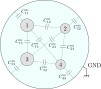
\includegraphics[width=\textwidth]{Figures/Electrodes/mutual_capacitance_scheme.pdf}
\end{minipage}
\begin{minipage}{0.48\textwidth}
	\begin{equation*}
	\Leftrightarrow \quad
	\bm{C}^m = 
	\begin{pmatrix}
	C_{11}^m & C_{12}^m & C_{13}^m & C_{14}^m \\ 
	C_{21}^m & C_{22}^m & C_{23}^m & C_{24}^m\\
	C_{31}^m & C_{32}^m & C_{33}^m & C_{34}^m \\
	C_{41}^m & C_{42}^m & C_{43}^m & C_{44}^m \\
	\end{pmatrix}
	\end{equation*}
\end{minipage}
\caption{Scheme representing an hypothetical electric modeling a system composed 3 electrodes $\{1,2,3\}$ surrounded by an electric ground $GND$. Each capacitance coupling corresponds to a term of the associated Mutual capacitance matrix. The diagonal terms $C_{ii}^m$ of the mutual capacitance matrix is called the self-capacitance and is modeled by a capacitance linking an electrode $i$ to the ground.}
\label{fig:lumped-capacitance}
\end{figure}

Each term $\bm{C}_{ij}^m$ can be interpreted as a single lumped capacitance between two electrodes $i$ and $j$ and as such, are represented with the common parallel-plate capacitor symbol. One can notice that the diagonal mutual capacitance terms $\bm{C}_{ii}^m$ are interpreted as the capacitance between the electrode $i$ and the ground (here the copper chassis). It is important to note that this matrix does not represent the relation between the electric charge $\vec{Q}$ and potential $\vec{V}$ of the electrodes of the system and therefore the equation \ref{eq:capacitance-definition-matrix} cannot be applied with the mutual capacitance matrix. Instead, the mutual capacitance matrix should be used as a modelization and interpretation tool. It is possible to obtain the Maxwell capacitance matrix from the mutual capacitance matrix according to the relations:

%\begin{equation} 
%\label{eq:mutual-to-maxwell}
%\bm{C} = 
%\begin{pmatrix}
%C_{11} & C_{12} & \cdots & C_{1N} \\ 
%C_{21} & C_{22} & \cdots & C_{2N} \\ 
%\vdots & \vdots & \ddots & \vdots \\ 
%C_{N1} & C_{N2} & \cdots & C_{NN}
%\end{pmatrix}
% = 
%\begin{pmatrix}
%\sum_{j=1}^N C_{1j}^m & -C_{12}^m & \cdots & -C_{1N}^m \\[0.3em]
%-C_{21}^m & \sum_{j=1}^N C_{2j}^m & \cdots & -C_{2N}^m \\[0.3em]
%\vdots & \vdots & \ddots & \vdots \\[0.3em] 
%-C_{N1}^m & -C_{N2}^m & \cdots & \sum_{j=1}^N C_{Nj}^m
%\end{pmatrix}
%\end{equation}

\begin{equation} 
\label{eq:mutual-to-maxwell}
\left\lbrace
\begin{array}{lc}
\forall i :& C_{ii} = \sum_j C_{ij}^m \\
\forall i \neq j:&  C_{ij} = - C_{ij}^m
\end{array}
\right.
\quad \Leftrightarrow \quad
\left\lbrace
\begin{array}{lc}
\forall i :& C_{ii}^m = \sum_j C_{ij} \\
\forall i \neq j:&  C_{ij}^m = - C_{ij}
\end{array}
\right.
\end{equation}

With the interpretation of the mutual matrix as lumped capacitances, we see that the diagonal terms $\bm{C}_{ii}$ of the Maxwell capacitance matrix are simply the equivalent capacitance to all the lumped mutual capacitance $\bm{C}_{ij}$ put in parallel $C_{ii} = \sum_{j=1}^N C_{ij}^m$. As the non-diagonal terms of the Maxwell and the mutual capacitance matrix are opposite, the mutual capacitance matrix is also symmetric.

COMSOL offers a functionality called Stationary Source Sweep to evaluate the elastance and the capacitance matrices. Considering the equation \ref{eq:elastance-matrix}, a terminal $j$ is excited with an electric charge $Q_j$ while the charges of all the other terminals $i\neq j$ are maintained to $Q_i=0$. The electrostatic system is numerically solved and the coefficient of potential can be deduced from the electric potential of the terminals $V_i$:
\begin{equation}
\bm{P_{ij}} = \frac{V_i}{Q_j}
\end{equation}
This procedure is repeated for each terminal until the full elastance matrix $\bm{P}$ is evaluated. The capacitance matrices are then calculated using the equations \ref{eq:maxwell-capacitance-matrix} and \ref{eq:mutual-to-maxwell}. In order to facilitate the discussion, the indexes of the matrices are swapped with the label of the electrodes. 

%In the case of the Planar38 design, the correspondence between indexes and label is:
%$$
%\{ \textsf{top}, \textsf{bottom} \} 
%\Leftrightarrow
%\{A,B\}
%\Leftrightarrow
%\{ 1, 2\}
%$$
For the PL38 detector design in its default configuration, the elastance and capacitance matrices are evaluated to:
\begin{equation} 
\label{eq:planar38-matrix-evaluation}
\begin{array}{rrccclc}
 & \bm{P} = &
 \begin{pmatrix}
P_{AA} & P_{AB} \\ 
P_{BA} & P_{BB}
\end{pmatrix}
&=&
\begin{pmatrix}
1.42 & 1.04 \\
1.04 & 1.42
\end{pmatrix}
& \cdot \SI{e11}{\per\farad} \\
\Rightarrow & \bm{C} = &
\begin{pmatrix}
C_{AA} & C_{AB} \\ 
C_{BA} & C_{BB}
\end{pmatrix}
&=&
\begin{pmatrix}
14.92 & -10.86 \\
-10.86 & 14.92
\end{pmatrix}
& \cdot \SI{e-12}{\farad} \\
\Rightarrow & \bm{C}^m = &
\begin{pmatrix}
C_{AA}^m & C_{AB}^m \\ 
C_{BA}^m & C_{BB}^m
\end{pmatrix}
&=&
\begin{pmatrix}
4.06 & 10.86 \\
10.86 & 4.06
\end{pmatrix}
& \cdot \SI{e-12}{\farad}
\end{array}
\end{equation}
 
As expected from a similarly designed parallel-plate capacitor using the equation \ref{eq:capacitor-basic}, the Mutual capacitance are close the tens of \si{\pico\farad}. As expected from the interpretation of the Mutual capacitance matrix, all of its terms are positive. Observing the Mutual capacitance matrix, we note that the capacitance between the electrodes $C_{AB}^m=\SI{10.86}{\pico\farad}$ is greater than the self-capacitance of the electrodes $C_{AA}^m = C_{BB}^m = \SI{4.06}{\pico\farad}$. According to the parallel-plate capacitor equation \ref{eq:capacitor-basic}, there are multiple arguments pointing towards an opposite observation: the grounded chassis is surrounding the electrodes, presenting very large area and the distance electrode-chassis is smaller than the height of the crystal. However, the self-capacitance is mainly formed in the vacuum between the absorber and the chassis, with a relative electric permittivity $\epsilon_r(\textsf{Vacuum})=1$ whereas the mutual capacitance between the electrodes $A$ and $B$ is forming in the germanium crystal which imposes a relative permittivity of $\epsilon_r(\textsf{Ge})=16.3$. This  significant difference in material permittivity explains the hierarchy of the mutual capacitance for the PL38 design.

%In the case of the FID38 design, the correspondence between indexes and labels is:
%$$
%\{ \textsf{Top Veto}, \textsf{Top Collect}, \textsf{Bottom Veto}, \textsf{Bottom Collect} \}
%\Leftrightarrow
%\{A,B,C,D\}
%\Leftrightarrow
%\{ 1,2,3,4\}
%$$
For the FID38 design with default parameters, the elastance and capacitance matrices are evaluated to:

\begin{equation} 
\label{eq:fid38-matrix-evaluation}
\begin{array}{rrccclc}
 & \bm{P} = &
 \begin{pmatrix}
P_{AA} & P_{AB} & P_{AC} & P_{AD} \\ 
P_{BA} & P_{BB} & P_{BC} & P_{BD} \\ 
P_{CA} & P_{CB} & P_{CC} & P_{CD} \\ 
P_{DA} & P_{DB} & P_{DC} & P_{DD}
\end{pmatrix}
&=&
\begin{pmatrix}
2.23 & 1.92 & 1.71 & 1.69 \\
1.92 & 2.34 & 1.69 & 1.68 \\
1.71 & 1.69 & 2.23 & 1.92 \\
1.69 & 1.68 & 1.92 & 2.34 \\
\end{pmatrix}
& \cdot \SI{e11}{\per\farad} \\
\Rightarrow & \bm{C} = &
\begin{pmatrix}
C_{AA} & C_{AB} & C_{AC} & C_{AD} \\ 
C_{BA} & C_{BB} & C_{BC} & C_{BD} \\ 
C_{CA} & C_{CB} & C_{CC} & C_{CD} \\ 
C_{DA} & C_{DB} & C_{DC} & C_{DD}
\end{pmatrix}
&=&
\begin{pmatrix}
18.25 & -10.19 & -4.02 & -2.58 \\
-10.19 & 15.94 & -2.58 & -1.98 \\
-4.02 & -2.58 & 18.25 & -10.19 \\
-2.58 & -1.98 & -10.19 & 15.94 \\
\end{pmatrix}
& \cdot \SI{e-12}{\farad} \\
\Rightarrow & \bm{C}^m = &
\begin{pmatrix}
C_{AA}^m & C_{AB}^m & C_{AC}^m & C_{AD}^m \\ 
C_{BA}^m & C_{BB}^m & C_{BC}^m & C_{BD}^m \\ 
C_{CA}^m & C_{CB}^m & C_{CC}^m & C_{CD}^m \\ 
C_{DA}^m & C_{DB}^m & C_{DC}^m & C_{DD}^m
\end{pmatrix}
&=&
\begin{pmatrix}
1.46 & 10.19 & 4.02 & 2.58 \\
10.19 & 1.18 & 2.58 & 1.98 \\
4.02 & 2.58 & 1.46 & 10.19 \\
2.58 & 1.98 & 10.19 & 1.18 \\
\end{pmatrix}
& \cdot \SI{e-12}{\farad} 
\end{array}
\end{equation}

The observations made previously for the PL38 design still holds for the FID38 design: capacitances are close to tens of \si{\pico\farad} and the self-capacitance term are the smaller terms. In particular, we note that the Mutual capacitance is dominated by the terms $C_{AB}^m=C_{BA}^m=C_{CD}^m=C_{DC}^m=\SI{10.19}{\pico\farad}$. Indeed, as the electrodes $A,B$ and $C,D$ are interleaved, their capacitive coupling is high as it emulates a situation with two close plates. The next higher term is $C_{AC}^m=\SI{4.02}{\pico\farad}$ coming from the two veto electrodes which are facing each other and coming very close to one another near the equator leading to an increase in coupling. The hierarchy of the remaining term can be explained by the fact that their are more veto electrode rings than collect electrode rings, thus emulating a higher electrode area in the equation \ref{eq:capacitor-basic}.


\subsection{Sensitivity Calculation}
\label{par:sensitivity-calculation}

%In the case of the FID38, we try to model the generation of the ionization signal. We consider an ideal detector with default parameters with no trapping and a single electron-hole pair created at a desired location. We assume that the electric charges will drift following exactly the electric field lines. The disposition of the electrodes for the FID38 design illustrated in the scheme \ref{fig:fid38-scheme} mentions four possible locations for the recoils to happen. Each location will have charges drifting towards a specific combination of electrodes inducing an electric charge perturbation $\vec{Q}$ according to the integration of the Shockley-Ramo theorem \ref{eq:ramo-theorem-integrated}.

The sensitivity of an electrode $X$ designated the amplitude of its voltage signal $V$ normalized by the ionization energy $E_{Ion.}$ created by a recoil. The unit of the sensitivity is the \si{\volt \per \kilo\eV}. In this paragraph, the sensitivities of each electrodes of the PL38 and FID38 design is calculated. The ionization signal is considered to be generated by an electronic recoil depositing an ionization energy $E_{Ion.} = E_R = \SI{1}{\kilo\eV}$. With application of the equation \ref{eq:number-pairs}, we deduce the average number of electron-hole pairs created $N_p = 1000/2.97 = 337$. The induced charge vectors $\vec{Q}$ were discussed in the paragraph \ref{par:stationnary-study}. The voltage signal vector $\vec{V}$ is computed using the relation \ref{eq:capacitance-definition-matrix}. For the sake of simplicity, this voltage signal $\vec{V}$ is normalized by \SI{1}{\kilo\eV} so that it equals the sensitivity.

In the case of the PL38 design, we refer to the equation \ref{eq:pl38-induced-charges} for the induced charge vectors. The sensitivity of the electrodes $A$ and $B$ to a recoil in the fiducial volume is:
\begin{equation}
\label{eq:planar38-sensitivity}
\vec{V}_{fid} = \bm{P} \vec{Q}_{fid} =
\begin{bmatrix}
- P_{AA} + P_{AB} \\ - P_{BA} + P_{BB}
\end{bmatrix}
\cdot N_p \cdot e
= 
\begin{bmatrix}
-0.39 \\  \\ 0.39
\end{bmatrix}
\cdot N_p \cdot e \cdot 10^{11}
= 
\begin{bmatrix}
-2.08 \\ 2.08 
\end{bmatrix}
\si{\micro\volt\per\kilo\eV}
\end{equation}

In the case of the FID38, we refer to the equation \ref{eq:fid38-induced-charges} for the four signature charge vectors. There are four corresponding voltage signal vectors:

\begin{align}
\label{eq:fid38-sensitivity}
\vec{V}_{bulk} = \bm{P} \vec{Q}_{bulk} &=
\begin{bmatrix}
- P_{AB} + P_{AD} \\
- P_{BB} + P_{BD} \\
- P_{CB} + P_{CD} \\
- P_{DB} + P_{DD} \\
\end{bmatrix}
\cdot N_p \cdot e
= 
\begin{bmatrix}
-0.23 \\ -0.66 \\ 0.23 \\ 0.66
\end{bmatrix}
\cdot N_p \cdot e \cdot 10^{11}
=
\begin{bmatrix}
-1.23 \\ -3.52 \\ 1.23 \\ 3.52
\end{bmatrix}
\si{\micro\volt\per\kilo\eV}
\\
\vec{V}_{veto, top} = \bm{P} \vec{Q}_{veto,top} &=
\begin{bmatrix}
+ P_{AA} - P_{AB} \\
+ P_{BA} - P_{BB} \\
+ P_{CA} - P_{CB} \\
+ P_{DA} - P_{DB} \\
\end{bmatrix}
\cdot N_p \cdot e
= 
\begin{bmatrix}
0.31 \\ -0.42 \\ 0.02 \\ 0.01
\end{bmatrix}
\cdot N_p \cdot e \cdot 10^{11}
= 
\begin{bmatrix}
1.65 \\ -2.24 \\ 0.11 \\ 0.05
\end{bmatrix}
\si{\micro\volt\per\kilo\eV}
\\
\vec{V}_{veto,bottom} = \bm{P} \vec{Q}_{veto,bottom} &=
\begin{bmatrix}
- P_{AC} + P_{AD} \\
- P_{BC} + P_{BD} \\
- P_{CC} + P_{CD} \\
- P_{DC} + P_{DD} \\
\end{bmatrix}
\cdot N_p \cdot e
= 
\begin{bmatrix}
0.02 \\ 0.01 \\ -0.31 \\ -0.42
\end{bmatrix}
\cdot N_p \cdot e \cdot 10^{11}
= 
\begin{bmatrix}
0.11 \\ 0.05 \\ -1.65 \\ 2.24
\end{bmatrix}
\si{\micro\volt\per\kilo\eV}
\\
\vec{V}_{equator} = \bm{P} \vec{Q}_{equator} &=
\begin{bmatrix}
- P_{AA} + P_{AC} \\
- P_{BA} + P_{BC} \\
- P_{CA} + P_{CC} \\
- P_{DA} + P_{DC} \\
\end{bmatrix}
\cdot N_p \cdot e
= 
\begin{bmatrix}
0.52 \\ 0.23 \\ -0.52 \\ -0.23
\end{bmatrix}
\cdot N_p \cdot e \cdot 10^{11}
= 
\begin{bmatrix}
2.77 \\ 1.23 \\ -2.77 \\ -1.23
\end{bmatrix}
\si{\micro\volt\per\kilo\eV}
\end{align}

The first thing one can note is that even though for each case the electron and hole were collected by two electrode, an electric potential perturbation was created on all the electrodes. This phenomenon is referred as "capacitive cross-talk". Then, we note that the amplitude of the signal depends on the electrode and depends of the event type.

% , referred as "electrode sensitivity" $S_{type}^{A} = |\vec{v}/e|$
% We can quantify this cross-talk by calculating the ratio $X_{type}$ between the signal induced on a non-collecting electrode over the signal induced on a collecting electrode:
%
%The sensitivity of an electrode corresponds to the amplitude of the voltage signal weighted by the input energy and is expressed in $\mu V/keV$. Considering the results of the equation \ref{eq:planar38-sensitivity} and \ref{eq:fid38-sensitivity}, for an electrode $X$ and a kind of event $type$, the sensitivity is expressed as:
%
%\begin{equation}
%S_{X, type} = | V_{X,type} | \quad \textsf{in} \quad [\mu V/keV]
%\end{equation}

%We can compare the FID38 design "efficiency" by comparing the Maxwell capacitance matrix, obtained in equations \ref{eq:planar38-matrix-evaluation} and \ref{eq:fid38-matrix-evaluation}, to a reference ideal two plate capacitance $C_{X, type}^{ref}$ of equal sensitivity that the considered event $type$ and electrode $X$. This reference capacitance is composed of a ground and a unique terminal such that the charge perturbation is $q_{ref}=-e$ and the induced electric potential $v_{ref}(type)$ is expressed as:

The sensitivity vector associated to the PL38 and FID38 designs possessing multiples electrodes are calculated. We can discuss the "efficiency" of the multiple electrodes design compared to a single equivalent reference capacitor. This reference capacitance $C_{X, type}^{ref}$ corresponds to a two-plate capacitor of same sensitivity as the electrode $X$ for a given event $type$. By applying the formula \ref{eq:capacitor-basic} for this reference capacitor, its capacitance is expressed as:
\begin{equation}
C_{X,type}^{ref} = \frac{N_p \cdot e}{| V_{X,type} |}
\end{equation}

%With the value of the sensitivity now calculated, we can define
%
%\begin{equation}
%C_{X,type}^{ref} = \left( \frac{| V_{X,type} |}{N_p \cdot e} \right)^{-1}
%\end{equation}

In the case of the PL38 detector, there is only one type of event (fiducial events) for two electrodes with equal sensitivities. The common reference capacitance is:

\begin{equation}
\label{eq:planar38-reference-capacitance}
C_{top}^{ref}
= C_{bottom}^{ref}
= \left( | -P_{AA} + P_{AB} |\right)^{-1}
= (0.39 \cdot 10^{11})^{-1}
= \SI{26e-12}{\farad}
\end{equation}

%The equivalent reference capacitance is 26 pF. 
It is greater than any term of the Maxwell or mutual capacitance matrices \ref{eq:planar38-matrix-evaluation} for the PL38 design. This indicates that this design has a worse efficiency than the two-plate capacitor design. The calculation of the sensitivity in equation \ref{eq:planar38-sensitivity} and the reference capacitance in equation \ref{eq:planar38-reference-capacitance} shows that the sensitivity is proportional to the term $| -P_{AA} + P_{AB} | = | -P_{AB} + P_{BB} |$. This term can be interpreted as the difference between the diagonal terms, $P_{AA}$ and $P_{BB}$, of the elastance matrix and the non-diagonal term $P_{AB}$ expressing the coupling between the two collecting electrodes.

As a \num{2 x 2} matrix, expressing the elastance $\bm{P}$ with the capacitance terms is relatively straightforward:
\begin{equation}
\bm{P} = \bm{C}^{-1} = 
\frac{1}{C_{11} C_{22} - (C_{12}^m)^2}
 \begin{pmatrix}
C_{22} & -C_{12} \\ 
-C_{12} & C_{11}
\end{pmatrix}
\end{equation}
The expression of the reference capacitance becomes:
\begin{equation}
C_{top}^{ref} = \left( | -P_{AA} + P_{AB} |\right)^{-1}
=  \frac{C_{11} C_{22} - (C_{12}^m)^2}{C_{22} + C_{12}}
= C_{11}^m + C_{12}^m \left( 1 + \frac{C_{11}^m}{C_{22}^m} \right)
\end{equation}
Considering the self-capacitance of $A$ and $B$ are almost equals, $C_{11}^m \approx C_{22}^m$, these expressions are simplified to:
\begin{equation}
\label{eq:pl38-ref-capa-expr}
C_{top}^{ref} = C_{22} - C_{12} = C_{22}^m + 2 C_{12}^m = \SI{25.78}{\pico\farad}
\end{equation}
In the end, in term of sensitivity, the electrodes $A$ and $B$ are equivalent to their self-capacitance $C_{22}^m$ in parallel with two coupling capacitance $C_{12}^m$. In a sens, this coupling capacitance has two times more effect on the sensitivity than the self-capacitance, which is detrimental here as the $C_{12}^m$ is the highest term of the mutual capacitance $\bm{C}^m$ of the PL38 design.

In the case of the FID38 detector, there are four types of events and four electrodes, resulting in a total of 16 sensitivities \ref{eq:fid38-sensitivity}. Among all these values, some are more relevant for the ionization channel performance than the others. The auxiliary veto electrodes $A,C$ are used to determine if an event is a bulk or veto event (see paragraph \ref{par:bulk-cut}). Therefore, the sensitivities of these veto electrodes are relevant in the case of $veto$ events of sensitivity $|V_{\textsf{veto top}, A}|=|V_{\textsf{veto bottom}, C}|$, and $equator$ events with $|V_{\textsf{equator}, A}|=|V_{\textsf{equator}, C}|$. The main electrodes $B,D$ are used to reconstruct the ionization energy $E_{Ion.}$ of the $bulk$ events. Thus, their sensitivities are relevant for $bulk$ recoils, $|V_{\textsf{bulk}, B}|=|V_{\textsf{bulk}, D}|$. From these sensitivities, the equivalent reference capacitances are deduced:

\begin{align}
C_{A, veto}^{ref} = C_{C, veto}^{ref}
= \left( | P_{AA} - P_{AB} |\right)^{-1}
= \left( | -P_{CC} + P_{CB} |\right)^{-1}
= (0.31 \cdot 10^{11})^{-1}
&= \SI{32e-12}{\farad}
\\
C_{A, equator}^{ref} = C_{C, equator}^{ref}
= \left( | P_{AA} - P_{AC} |\right)^{-1}
= \left( | -P_{CC} + P_{AC} |\right)^{-1}
=(0.52 \cdot 10^{11})^{-1}
&= \SI{19e-12}{\farad}
\\
C_{B, bulk}^{ref} = C_{D, bulk}^{ref}
= \left( | -P_{BB} + P_{BD} |\right)^{-1}
= \left( | P_{DD} - P_{BD} |\right)^{-1}
= (0.66 \cdot 10^{11})^{-1}
&= \SI{15e-12}{\farad}
\end{align}

With a reference capacitance of \SI{32}{\pico\farad}, the same observation as for the FID38 can be made for the veto electrode $A$ and $C$ in their sensitivity to $veto$ events. The reference capacitance is higher than any term of the mutual capacitance $\bm{C}^m$ or the diagonal term of the Maxwell capacitance $\bm{C}$. The efficiency of these electrodes is worse than a basic two-plate capacitor.

In the case of the $equator$ events however, the reference capacitance $C_{A, equator}^{ref}$ seems to corresponds to the diagonal term of the Maxwell matrix $C_{AA}=\SI{18.25}{\pico\farad}$. Similarly, the reference capacitance $C_{B, bulk}^{ref}$ associated with the electrode $B$ and $D$ for $bulk$ events is close to $C_{BB} = \SI{15.94}{\pico\farad}$. In other words, for these two instances, an electrodes is as sensitive as the parallel association  of all of its associated mutual capacitances.

Further interpretation of the reference capacitance and sensitivity is hampered due to the higher dimensions \num{4 x 4} of the elastance matrix $\bm{P}$ of the FID38 design. An analytical expression of the reference capacitance like for PL38 in equation \ref{eq:pl38-ref-capa-expr} is not easily accessible and should prove to be much more complex.


% Comment these values

There is a specific cross-talk and sensitivity for each type of events. When analyzing the detector data, there should therefore be a specific calibration and cross-talk correction associated to each of this type of signal.
However, to this day, the EDELWEISS and R\&D experiments have only use a single analysis pipeline with a single calibration value for each electrodes and a single cross-talk correction matrix, independently of the type of event. Furthermore, the analysis seemed valid and no significant deviation was observed from the simple, yet wrong, ionization model where events creating the same amounts of electron-hole pairs presents the same electrode sensitivity and capacitive cross-talk. This can be explained by the fact that the capacitances of the detector are dominated by the greater capacitance of the cabling. It is important to recall that this work is focused on the capacitance of the electrodes of a detector, and did not considered the capacitance of the cabling between the electrodes and the amplifying electronics. In the experimental setup, the electrodes are cabled to the electronics with coaxial cables. While a coaxial cable shield the signal from exterior interferences, it also creates a significant capacitive coupling between the ground and the core (in this case, the electrode). Let's consider a of \SI{50}{\pico\farad} capacitance between the ground and each electrodes, the associated cabling capacitance matrix are:
\begin{equation}
\bm{C}_{cabling} = \bm{C}_{cabling}^m = \mathbb{1} \SI{50e12}{\farad}
\end{equation}
As the Maxwell matrix $\bm{C}_{cabling}$ is diagonal, it is equal to the mutual matrix $\bm{C}_{cabling}^m$. The total Maxwell and mutual capacitance matrices of the detector and cabling are given by:
\begin{equation}
\begin{cases} 
\bm{C}_{cabling} &= \bm{C}_{detector} + \bm{C}_{cabling} \\
\bm{C}_{cabling}^m &= \bm{C}_{detector}^m + \bm{C}_{cabling}^m
\end{cases}
\end{equation}
where $\bm{C}_{detector}$ and $\bm{C}_{detector}^m$ are the Maxwell and mutual capacitance matrices of the detector designs PL38 and FID38 evaluated in the equations \ref{eq:planar38-matrix-evaluation} and \ref{eq:fid38-matrix-evaluation} respectively.
The elastance matrices of the detectors and the cabling is now evaluated to:

\begin{equation}
\bm{P}_{tot}^{PL38}
=
\begin{bmatrix}
  0.158 & 0.027 \\
  0.027 & 0.158 \\
\end{bmatrix}
\cdot
\SI{e11}{\per\farad}
\quad \quad
\bm{P}_{tot}^{FID38} = 
\begin{bmatrix}
  0.151 & 0.024 & 0.011 & 0.008\\
  0.024 & 0.156 & 0.008 & 0.007\\
  0.011 & 0.008 & 0.151 & 0.024\\
  0.008 & 0.007 & 0.024 & 0.156\\
\end{bmatrix}
\cdot \SI{e11}{\per\farad}
\end{equation}

For the PL38 design with the capacitive cabling, the sensitivity and associated reference capacitance are now:
\begin{equation}
\vec{V}_{event}
=
\begin{bmatrix}
0.131 \\
-0.131
\end{bmatrix}
\cdot 10^{11}
=
\begin{bmatrix}
0.71 \\
-0.71
\end{bmatrix}
\si{\micro\volt\per\kilo\eV}
\end{equation}

\begin{equation}
C_{top, bottom}^{ref}
= 0.131 \cdot 10^{11}
= \SI{76e-12}{\farad}
\end{equation}

In the case of the FID38 with the capacitive cabling:

\begin{align}
\label{eq:fid38-cabling-sensitivity}
\vec{V}_{bulk}
=
\begin{bmatrix}
  -0.016 \\ -0.149 \\ 0.016 \\ 0.149\\
\end{bmatrix}
\cdot 10^{11}
= &
\begin{bmatrix}
-0.05 \\ -0.80 \\ 0.05 \\ 0.80
\end{bmatrix}
\si{\micro\volt\per\kilo\eV}
\\
\vec{V}_{veto,top}
=
\begin{bmatrix}
  0.127 \\ -0.132 \\ 0.003 \\ 0.001\\
\end{bmatrix}
\cdot 10^{11}
= &
\begin{bmatrix}
0.69 \\ -0.75 \\ 0 \\ 0
\end{bmatrix}
\si{\micro\volt\per\kilo\eV}
\\
\vec{V}_{veto,bottom}
=
\begin{bmatrix}
  -0.003 \\ -0.001 \\ -0.127 \\ 0.132\\
\end{bmatrix}
\cdot 10^{11}
= &
\begin{bmatrix}
0 \\ 0 \\ -0.69 \\ 0.75
\end{bmatrix}
\si{\micro\volt\per\kilo\eV}
\\
\vec{V}_{equator}
=
\begin{bmatrix}
  0.140 \\ 0.016 \\ -0.140 \\ -0.016\\
\end{bmatrix}
\cdot 10^{11}
= &
\begin{bmatrix}
0.75 \\ 0.05 \\ -0.75 \\ -0.05
\end{bmatrix}
\si{\micro\volt\per\kilo\eV}
\end{align}

\begin{align}
C_{A, veto}^{ref} = C_{C, veto}^{ref}
= 0.127 \cdot 10^{11}
&= \SI{78.7e-12}{\farad}
\\
C_{A, equator}^{ref} = C_{C, equator}^{ref}
= 0.140 \cdot 10^{11}
&= \SI{71.4e-12}{\farad}
\\
C_{B, bulk}^{ref} = C_{D, bulk}^{ref}
= 0.149 \cdot 10^{11}
&= \SI{67.1e-12}{\farad}
\end{align}

We see that by adding the capacitance of the cabling, the cross-talk phenomenon is significantly lessened: the self-capacitance term $\bm{C}^m_{tot}$ dominates the mutual matrix and heavily influence the calculation of the elastance matrix $\bm{P}_{tot}$. The electrode sensitivities all tends to a unique value of $\approx \SI{75}{\pico\farad}$ in absolute value for all the types of events. This unified sensitivity is characteristic of the results yielded by the ionization channel of the EDELWEISS-II experiment and IP2I R\&D. The high cabling capacitance muffles the cross-talk phenomenon and the differences in sensitivity. Indeed as the capacitive coupling with the ground through the coaxial cabling is increased, the cross-talk and difference in sensitivity vanish.

In order to fully appreciate the impact of the cabling capacity, the figure \ref{fig:predict-corner-plot} presents the corner plot of the sensitivity vectors in a FID38 detector with (black points) and without (colored points) \SI{150}{\pico\farad} cabling capacitance.

\begin{figure}
\centering
%\includegraphics[width=\linewidth]{Figures/Electrodes/predict_corner_plot.png}
\includegraphics[width=\linewidth]{Figures/Electrodes/pl38_predictive_sensitivity.pdf}
\caption{Illustration of the expected sensitivities with a FID38 detector with ("w/ \SI{150}{\pico\farad}" black circles) and without ("w/ \SI{0}{\pico\farad}" color squares) capacitive cabling. The rectangular-like shape formed by the sensitivities of the FID38 with cabling is characteristic of the current IP2I R\&D results.}
\label{fig:predict-corner-plot}
\end{figure}
%There are 1000 points for each event types, and each channel is modeled by a gaussian distribution of variance 100eV.

The first major observation is that the cabling capacitance drastically reduce the sensitivities of the electrodes. Then, the sensitivities of the FID38 with cabling forms a square-like pattern in the $V_B(V_D), V_C(V_D), V_B(V_A), V_C(V_A)$ subplots illustrating that all electrode have almost the same sensitivity.  The square pattern emerges from the low cross-talks of about $0.05/0.80=\SI{6}{\percent}$ and $0.05/0.75=\SI{7}{\percent}$. This pattern is redundant in the data analysis of the EDELWEISS-III and IP2I R\&D data streams (see later chapter \ref{ChapterElectrodesExperimental} discussing the data analysis). 
In the case of EDELWEISS-III with a cabling of capacitance $>\SI{150}{\pico\farad}$, the simple ionization signal generation model of this chapter introduction \ref{eq:capacitor-basic} is sufficient to explain their experimental observations. The eventual low cross-talks phenomenon were absorbed in the ionization resolution or attributed to unknown parasite capacitance in the electronics.

The new HEMT-based electronics in development is situated very close to the detector load in the cryostat. This implies a reduced coaxial cable length and a lowered cabling capacitance. The major advantage is a significant gain in sensitivity, which was expected and now demonstrated in this study. The novelty brought with this theorization of the ionization channel is that with low cabling capacitance, the signal on the electrodes will differ. The 4 events populations do not form a square pattern anymore and presents the high cross-talk phenomenon $1.23/3.52=\SI{35}{\percent}$ and $1.23/2.77=\SI{44}{\percent}$.


\subsection{Noise and Resolution Calculation}
\label{par:ion-resolution-calculation}

The previous paragraph presented how, with low cabling capacitance, the capacitive coupling between each electrodes affects the sensitivity of the ionization channel. This paragraph discusses the impact of this capacitive coupling on the noise affecting the measurement and eventually the resolution of the ionization channel. A discussed in the previous paragraph \ref{par:electronics-ionization}, the dominating noise source affecting the ionization energy measurement is the electronics noise. By combining the electric circuit of the HEMT-based electronics line and the lumped capacitance model \ref{fig:lumped-capacitance} of the PL38 and FID38 designs, we can predict the noise affecting the ionization channel. The method of noise propagation is the same as used in the chapter \ref{ChapterEthem} with the modelization of the heat channel.

%A previous paragraph \ref{par:electronics-ionization} already presented the noise propagation and resolution calculation for the future HEMT electronics. These calculations were based on a single HEMT line cabled on a single capacitance $C_d$ representing an electrode of the detector. We will now study how the noise calculation is affected by the coupling of multiple HEMT lines.
%
%{\color{blue} Discussion on the Hemt (see JB notes or Alex paper. Expected resolution and noise.}
%Explaining how to propagate the noise through the hemt line (superposition theorem, thevenin-norton transformation). Presented and illustrated in the figure \ref{fig:hemt-performances}.
%Simple model: Single hemt/electrode with a single detector capacitance (previously thought to be the diagonal term of the Maxwell capacitance matrix).

In order to motivate this study, the noise calculation is first done on a very simple model: the PL38 design with a heavily simplified HEMT line featuring only the polarization resistor $R_{polar.}$ and its associated Johnson noise $e_J$. The LPSD associated with the Johnson noise is expressed as:
\begin{equation}
e_J = \sqrt{4 \cdot T \cdot R_{polar.}}
\end{equation}
with the temperature of the polarization resistor set to $T=\SI{20}{\milli\kelvin}$. The scheme of this simplified model is presented in the figure \ref{fig:scheme-planar38-simplified}. Thanks to the superposition theorem and successive Thevenin-Norton transformations of the electric circuit, it is possible to propagate the two Johnson noise source $e_{J,A}$ and $e_{J,B}$ to the measurement point $S_B$. 

The voltage noise affecting the measurement at the node $S_B$ is characterized by the LPSD $e_{tot}^{S_B}$ in \si[per-mode=symbol]{\volt\per\sqrthz}. It is expressed as:
\begin{equation}
\left( e_{tot}^{S_B} \right)^2
=
e^{S_B} \left( e_J^A \right)^2
+
e^{S_B} \left( e_J^B \right)^2
\end{equation}
with the components $e^{S_B} (\textsf{source})$ being the propagation of the different noise sources onto the node $S_B$.

% noise propagation
The propagation of the noise is done with multiple Thevenin-Norton transformations of the electric circuit. We use the parallel operator $\parallel$ to express the parallel association of two impedance $Z_1$ and $Z_2$ such that:
\begin{equation}
Z_1 \parallel Z_2 = \left( \frac{1}{Z_1} + \frac{1}{Z_2} \right)^{-1} = \frac{Z_1 \cdot Z_2}{Z_1 + Z_2}
\end{equation}

In the case of the simplified electric circuit representing the PL38 design, the propagation of the Johnson voltage noises $e_J$ onto the node $S_B$ are expressed:
\begin{align}
e^{S_B} \left( e_J^B \right)
&=
e_J^B
\cdot 
\frac{1}{R_{polar.}}
\cdot
\left( R_{polar.} \parallel (j\omega C_{22}^m)^{-1} \parallel Z_{eq} \right)
\\
e^{S_B} \left( e_J^A \right)
&=
e_J^A
\cdot
\frac{R_{polar.} \parallel (j\omega C_{11}^m)^{-1} }{R_{polar.} \cdot Z_{eq}}
\cdot
\left( R_{polar.} \parallel (j\omega C_{22}^m)^{-1} \parallel Z_{eq} \right)
\end{align}

and with the equivalent impedance $Z_{eq}$ expressed as:
\begin{equation}
Z_{eq}
=
\left( R_{polar.} \parallel (j \omega C_{11}^m)^{-1} \right) + (j \omega  C_{12}^m)^{-1}
=
\frac{1 + j \omega R_{polar.} ( C_{11}^m + C_{12}^m )}{(1 + j\omega R_{polar.} C_{11}^m) \cdot j\omega C_{12}^m}
\end{equation}
%=\frac{R_{polar.}}{1 + j \omega R_{polar.} C_{11}^m} + \frac{1}{j \omega C_{12}^m}

As a result, the ratio of the components is:
\begin{equation}
\begin{split}
\left\vert
\frac{
e^{S_B} \left( e_J^A \right)
}{
e^{S_B} \left( e_J^B \right)
}
\right\vert
&=
\left\vert
\frac{R_{polar.} \parallel (j\omega C_{11}^m)^{-1} }{R_{polar.} \cdot Z_{eq}}
\right\vert
\\
&=
\left\vert
\frac{R_{polar.}}{1 + j \omega R_{polar.} C_{11}^m}
\cdot 
\frac{(1 + j\omega R_{polar.} C_{11}^m) \cdot j\omega C_{12}^m}{1 + j \omega R_{polar.} ( C_{11}^m + C_{12}^m )}
\right\vert
\\
&=
\left\vert
\frac{ j \omega R_{polar} C_{12}^m }{ 1 + j \omega R_{polar} \left( C_{12}^m + C_{11}^m \right) }
\right\vert
\end{split}
\end{equation}

This ratio is consistent with a high-pass filtering assured by the coupling capacitance $C_{12}$. The asymptotic value of the ratio is:
\begin{equation}
\label{eq:planar38-analytical}
\lim_{\omega \to \infty}
\left\vert
\frac{
e^{S_B} \left( e_J^A \right)
}{
e^{S_B} \left( e_J^B \right)
}
\right\vert
=
  \frac{ C_{12}^m }{ C_{12}^m + C_{11}^m }
=
  \frac{ -C_{12} }{ C_{11} }
=
  \frac{ \SI{10.86}{\pico\farad} }{ \SI{14.92}{\pico\farad} }
=
  0.7279
\end{equation}

The cutoff frequency $f_c$ associated with this ratio function is calculated as:
\begin{equation}
\label{eq:planar38-cutoff}
\begin{split}
&
\left\vert
\frac{
e^{S_B} \left( e_J^A \right)
}{
e^{S_B} \left( e_J^B \right)
}
\right\vert
(\omega = \omega_c)
=
\frac{1}{\sqrt{2}}
\lim_{\omega \to \infty}
\left\vert
\frac{
e^{S_B} \left( e_J^A \right)
}{
e^{S_B} \left( e_J^B \right)
}
\right\vert
\\
\Leftrightarrow \quad &
\frac{ j \omega_c R_{polar} \left( C_{12}^m + C_{11}^m \right) }{ 1 + j \omega R_{polar} \left( C_{12}^m + C_{11}^m \right) }
=
\frac{1}{\sqrt{2}}
\\
\Leftrightarrow \quad &
\omega_c = \frac{1}{R_{polar} \left( C_{12}^m + C_{11}^m \right)} = \SI{6.702}{\radian\per\s}
\\
\Leftrightarrow \quad &
f_c = \frac{\omega_c}{2\pi} = \SI{1.067}{\Hz}
\end{split}
\end{equation}

The total noise and its components measured at $S_B$ are plotted as functions of the frequency in the top subplot of figure \ref{fig:planar38-analytical-results}. Event though the original Johnson voltage noise source are modeled as white noise whose levels are independent from the frequency, the total voltage noise affecting the measurement at node $S_B$ presents a low-pass filter profile. This is consistent with the studied electric system as the node $S_B$ is linked to the electric ground through the two capacitors $C_{22}$ and $C_{11}$: at high frequency, they act as closed circuit and the electric potential of the node $S_B$ tends to \SI{0}{\volt}. The dominant component of the noise is the Johnson noise $e_{J,B}$ of the HEMT line of the electrode $B$ where the measurement is made. It is less dampened than the other Johnson noise source $e_{J,A}$ which is filtered by the capacitance $C_{12}$ coupling the two electrodes $A$ and $B$. The bottom subplot of figure \ref{fig:planar38-analytical-results} shows the ratio of the two Johnson noise components $e_{J,A}/e_{J,B}$ as a function of the frequency.

\begin{figure}
\centering
\includegraphics[scale=1]{Figures/Electrodes/pl38_analytical_noise_propagation.pdf}
\caption{The top subplot presents the total voltage noise LPSD measured at the node $S_B$ along with its to propagated Johnson noise components as functions of the frequency. The bottom subplots compares these two components by plotting their ratio as a function of the frequency.
}
\label{fig:planar38-analytical-results}
\end{figure}

Above the cutoff frequency $f_c = \SI{1.067}{\Hz}$, the ratio tends to $0.73$. As the time windows is \SI{1}{\s}, the lowest frequency explored is \SI{1}{\Hz} which is very close to $f_c$. As such, the ratio is its asymptotic behavior on almost the whole frequency space. According to the previous equation \ref{eq:planar38_analytical}, the ratio depends on the ratio of the non-diagonal over the diagonal terms of the Maxwell capacitance matrix of the Planar38 detector (from equation \ref{eq:planar38-matrix-evaluation}). This ratio of Maxwell capacitance is comprised between 0 and 1, and reaches its maximum if the capacitive coupling $C_{12}^m$ between the two electrodes $A$ and $B$ is much greater than the self-capacitance $C_{11}^m$ of the electrode $A$.

As the two Johnson noise are not correlated, their squared noise level is added to form the total noise level which is tends to be $\sqrt{1^2 + (0.73)^2} = 1.24$ times the original Johnson noise level caused by $e_{J,B}$ alone. With the given PL38 design with the simplified HEMT line, the noise level is increased by \SI{24}{\percent} on the majority of the frequency space. This demonstrates that the effect of the coupling between the electrodes is far from negligible and should be properly studied for the two reference designs FID38 and PL38 with a full model with a complete HEMT line on each of the electrode.

\begin{landscape}

\begin{figure}
\centering
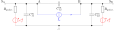
\includegraphics[scale=1]{Figures/Electrodes/pl38_analytical_circuit.pdf}
\caption{Electric scheme of the PL38 design with its two electrodes $A$ and $B$ solely equipped with the polarization line. The lumped capacitance model is used to model the PL38 design as an association of capacitors. Their capacitance corresponds to the term of the mutual capacitance matrix $C^m$ of the PL38 design. The transient signal sources are colored blue while the noise source are in red.}
\label{fig:pl38-analytical-circuit}
\end{figure}

\begin{figure}
\centering
\includegraphics[scale=1]{Figures/Electrodes/pl38_full_circuit.pdf}
\caption{Electric scheme of the PL38 design with its two electrodes $A$ and $B$ equipped with an HEMT line readout. The lumped capacitance model is used to model the PL38 design as an association of capacitors. Their capacitance corresponds to the term of the mutual capacitance matrix $C^m$ of the PL38 design. The transient signal sources are colored blue while the noise source are in red.}
\label{fig:pl38-full-circuit}
\end{figure}

\end{landscape}

\begin{table}[]
\centering
%\resizebox{\textwidth}{!}{%
\begin{tabular}{l c S}
Circuit Component		                    & Symbol        & {Value} \\
\hline \hline
Parasite Capacitance                        & $C_p$         & \SI{5e-12}{\farad}  \\
Polarization Resistance                     & $R_{polar}$   & \SI{1e10}{\ohm}    \\
Coupling Capacitance                        & $C_{c}$       & \SI{2e-9}{\farad}     \\
HEMT Capacitance                            & $C_{hemt}$    & \SI{5e-12}{\farad}   \\
Feedback Resistance                         & $R_{fb}$      & \SI{1e10}{\ohm}    \\
Feedback Capacitance                        & $C_{fb}$      & \SI{3e-12}{\farad}
\end{tabular}
%}%
\caption{List and Values of the electrical components of the circuits \ref{fig:scheme-planar38-simplified}, \ref{fig:scheme-planar38-full}, \ref{fig:scheme-fid38-fat} and \ref{fig:scheme-fid38-redux}.}
\label{tab:lcapy-components}
\end{table}

The PL38 detector cabled with the full HEMT line is illustrated in the scheme \ref{fig:scheme-planar38-full}. The detector is composed of the three mutual capacitance $C_{ij}^m$ linked to the nodes $A,B$. There is a measurement node for each electrode $S_A$ and $S_B$, acting as an ideal voltmeter with the electric ground as reference. There is a total of 6 noise sources coming from the HEMT lines. The signal induced by an event is modeled as a transient current source $I_{event}=N_p \cdot e \cdot \delta(t)$ between $A$ and $B$. The intrinsic current $i_n$ and voltage $e_n$ source of the amplifying electronic have their LSPD modeled as:
\begin{equation}
\begin{cases}
i_n(f) &= \sqrt{ i_0^2 +(i_a \cdot \sqrt{f})^2 } \\
i_0 &= \SI{4.0e-23}{\ampere} \\
i_a &= \SI[per-mode=symbol]{2.6e-18}{\ampere\per\sqrthz} \\
e_n(f) &= \sqrt{ e_0^2 +(\frac{e_a}{\sqrt{f}})^2 } \\
e_0 &= \SI{2.2e-10}{\volt} \\
e_a &= \SI[per-mode=symbol]{3.6e-8}{\volt\per\sqrthz}
\end{cases}
\end{equation}
with $f$ the frequency, based on experimental measurements.
% ref JB, Young
The multiple noise source and the event signal are propagated to the measurement node $S_B$ using the analytical circuit resolution algorithm from the Python module "Lcapy".
% (see Lcapy module for Python).
% Noise propagation plot
The figure \ref{fig:planar38-propagation} presents the total noise and its components measured at $S_B$ as a function of the frequency. The predominant noises are the Johnson noise $e_{J}^B$ of the Hemt line of the electrode $B$ at low frequency and the intrinsic current noise $i_n^B$ at high frequency. The Johnson noise $e_J^A$ from the other HEMT line of the electrode $A$ is slightly present below \SI{2}{\Hz}, but is surpassed by the intrinsic voltage source $e_n^B$. In the end, we observe that the noise sources from the auxiliary HEMT line on $A$ are heavily filtered and does not propagate significantly to the measurement node $S_B$. When comparing to the previous simplified electric circuit where the propagation was significant, one of the main difference is now the presence of the feedback capacitance, the HEMT intrinsic capacitance and the cabling capacitance (representing in this case 5+3+5 = \SI{13}{\pico\farad}. These capacitances are added to the diagonal term of the Maxwell capacitance matrix and reduce the propagation of the noise source through the coupling capacitance $C_{12}^m$.

\begin{figure}
\centering
\includegraphics[scale=1]{Figures/Electrodes/pl38_noise_propagation.pdf}
\caption{Representation of the total voltage noise LPSD the node $S_B$ along with its components as functions of the frequency. The signal power spectrum represented with the the alternative right. The calculation and integration from \SI{1}{\Hz} of the noise equivalent power yields the ionization energy resolution $\sigma_{B} = \SI{34}{\eV}$.}
\label{fig:planar38-propagation}
\end{figure}

% Noise vs Signal
The figure \ref{fig:planar38-propagation} also compares the total noise power spectral density to the power spectrum of the signal induced by the transient $I_{bulk}$. The noise follows a $1/\sqrt{f}$ trend while the signal has $1/f$ profile. As such, the majority of the information of the signal is contained in the low frequency of the data stream. When integrating between \SI{1}{\Hz} and infinity, the ionization energy resolution is evaluated to $\sigma_B=\SI{33.97}{\eV}$. There is factor 3 between this predicted resolution and the naive objective resolution of \SI{10}{\eV} discussed in the paragraph \ref{par:ionization-objective}. By combining the signal of the two electrodes, a lower resolution $\sigma_{A+B} = \sigma_B / \sqrt{2} = \SI{24.02}{\eV}$ is reached. 
%(bad? Can be compared to the initial simple model with a single Hemt and single electrode equivalent to the detector).


% FID38 noise propagation
The FID38 detector cabled with the full HEMT line is illustrated in the scheme \ref{fig:scheme-planar38-full}. The detector is composed of the ten mutual capacitance $C_{ij}^m$ linked to the nodes $A,B,C,D$. There is a measurement node for each electrode $S_A, S_B, S_c, S_D$, acting as an ideal voltmeter with the electric ground as reference. There is a total of $4\times3=12$ noise sources coming from the four HEMT lines. Signals induced by the $bulk$, $veto$ and $equator$ events are modeled as transient current sources $I=N_p \cdot e \cdot \delta(t)$ between two electrode nodes. Once again, the multiple noise source and the event signals are propagated to the measurement node $S_B$.

\begin{landscape}

\begin{figure}
\centering
\includegraphics[scale=1]{Figures/Electrodes/fid38_full_circuit.pdf}
\caption{Electric scheme of the FID38 design with its four electrodes $A$, $B$, $C$ and $D$ each equipped with an HEMT line readout. The lumped capacitance model is used to model the FID38 design as an association of capacitors. Their capacitance corresponds to the term of the mutual capacitance matrix $C^m$ of the FID38 design. The transient signal sources are colored blue while the noise source are in red.}
\label{fig:fid38-full-circuit}
\end{figure}

\begin{figure}
\centering
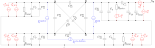
\includegraphics[scale=1]{Figures/Electrodes/fid38_reduced_circuit.pdf}
\caption{Simplification of the previous electric scheme \ref{fig:fid38-full-circuit} for the calculation of the sensitivity and the propagation of the noise on the readout of the electrode $B$.}
\label{fig:fid38-reduced-circuit}
\end{figure}

\end{landscape}

% Noise propagation plot
The figure \ref{fig:fid38-propagation} presents the total noise and its components measured at $S_B$ as a function of the frequency. The predominant noise are the Johnson noise $e_{J,B}$ of the HEMT line of the electrode $B$ at low frequency and the intrinsic current noise $i_n^B$ at high frequency. The Johnson noise $e_J^A$ from the other HEMT line of the electrode $A$ is slightly present below \SI{2}{\Hz}, but is quickly dominated by the intrinsic voltage source $e_n^B$. All in all, the results are quite similar to what was observed with the PL38 design: the Johnson noise from the most coupled electrode is significant at very low frequency and is quickly dominated by the intrinsic voltage noise source of the HEMT line $B$. Again, this can be explained by a boosted diagonal term in the Maxwell capacitance matrix which heavily filter the noise sources from spreading to other HEMT line efficiently.
% Noise vs Signal
In the case of the FID38, there are three possible signal power spectrum associated with the $bulk$, $veto$ and $equator$ events. All this power spectrum have the same $1/f$ profile and only differ by a multiplicative factor.
Once again, due to the $1/\sqrt{f}$ shape of the total noise, most of the information is held in the low frequency of the data stream. The ionization energy resolution are calculated from the three event types. For the bulk and veto events, the resolutions are pretty similar around \SI{30}{\eV} while the resolution associated with the equator events is very high \SI{151}{\eV}. This indicates that the performance of the FID38 ionization channel drops for equatorial events. This might be problematic in tagging surface events near the equator. The lowest resolution concerns the bulk events with $\sigma_{bulk}^B = \SI{28.4}{\eV}$. By combining the two collecting signal of the collecting electrodes $B$ and $D$, it is possible to lower the ionization energy resolution to  $\sigma_{bulk}^{B+D} = \SI{20.1}{\eV}$. Even if this resolution is two times superior to the objective \SI{10}{\pico\farad}, it is still very close.

\begin{figure}
\centering
\includegraphics[scale=1]{Figures/Electrodes/fid38_noise_propagation.pdf}
\caption{Representation of the total voltage noise LPSD the node $S_B$ along with its components as functions of the frequency. The signal power spectrum associated with the $bulk$, $veto$ and $equator$ events are represented with the the alternative right. The calculation and integration from \SI{1}{\Hz} of the noise equivalent power yields the ionization energy resolutions.
}
\label{fig:fid38-propagation}
\end{figure}

% Planar38 Scan
The performance of a detector is partly quantified by the resolution of its ionization channel. Thus, the resolutions calculated previously for the PL38 and FID38 are figure of merits. However, these calculation are long as they necessitate to simulate a detector design in the FEM software to compute the Mutual capacitance matrix and then simulate the detector cabled with the HEMT lines with a separate Python script using the Lcapy module.

The resolution of the electrodes of a detector design depends on the whole Maxwell capacitance matrix (3 independent terms for the PL38, and 10 independents terms for the FID38). It might be possible to access some basic trends of the resolution by scanning over basic parameters.

The left figure \ref{fig:planar38-scan} is a graph of the calculated resolution as a function of the cabling capacitance $C_p$ of the HEMT lines while keeping fixed all the other component values \ref{tab:lcapy-components}. This parameter scan can be interpreted as studying the resolution as a function of the diagonal terms of the Maxwell capacitance terms. We observe that a high cabling capacitance increases the resolution of the ionization channel. As the cabling capacitance decreases, the resolutions seem to cap. This indicates that $C_p$ is not the limiting component in the detector under $\approx \SI{5}{\pico\farad}$

The right figure \ref{fig:planar38-scan} is a graph of the resolution as a function of a global multiplier factor of the Maxwell capacitance matrix for the PL38 design. The Maxwell capacitance $\bm{C}_{new}$ used for the resolution calculation is:
\begin{equation}
\bm{C}_{new} = \bm{C} \times \alpha
\end{equation}
with $\alpha$ the multiplicative factor. A multiplier factor of 1 corresponds to a resolution calculation with the presented capacitance matrices presented in the equation \ref{eq:planar38-matrix-evaluation}. It is possible to artificially change all the capacitance terms of the capacitance matrix with this global multiplier factor. Compared to the previous scan on the diagonal term of the Maxwell matrix, this scan impact the whole matrix. In order to realistically apply this transformation, we could think of a up or down-scaling of the detector size or changing the electric permittivity with another absorber material. We observe that the resolution is proportional to the global multiplier factor.

\begin{figure}
\centering
\includegraphics[scale=1]{Figures/Electrodes/pl38_scanplot.pdf}
\caption{Ionization energy resolutions of the PL38 design as functions of the cabling capacitance $C_p$ of the HEMT line and the global multiplicative factor $\alpha$ of the detector Maxwell matrix. The blue curve corresponds to the resolution of the single collect electrode $B$. The orange curves corresponds to the combination of the signal from $B$ and $D$ inducing a gain of factor $1/\sqrt{2}$ on the initial resolution.
}
\label{fig:planar38-scan}
\end{figure}

These two observations are consistent with what could be expected from the very basic understanding of the ionization channel presented in the paragraph \ref{par:basic-ion-channel}: the resolution decreases as the capacitances of the detector decrease. 
In order to optimize the ionization channel, the research should be focused on lowering the capacitance of the cabling, and lowering the capacitances of the electrodes.
The cabling links the electrodes evaporated on the germanium crystal and the HEMT electronics. Its capacitance depends on the type of cabling (shielded, material) and is proportional to its length. As a result, lowering the cabling capacitance is ultimately a geometric challenge on the cryostat configuration and the suspended tower. Currently, the cabling capacitance is guaranteed to be lower than \SI{20}{\pico\farad}. As discussed, this would still limit the ionization resolution. With further research on the placement of the HEMT-based electronics in the cryostat lower could be reached. If the cabling capacitance goes to \SI{5}{\pico\farad}, it is not the limiting factor for the resolution anymore, the capacitance of the electrodes become limiting. These capacitance depends on the design of the detector and is heavily discussed in the chapter \ref{ChapterElectrodesScan}.
